\chapter{传播信号:动作电位} \label{chap:chap10}

神经细胞能够远距离传输电信号,因为远距离信号(动作电位)会不断再生,因此不会随着轴突向下移动而衰减。 
在第~\ref{chap:chap9}~章中,我们了解了膜对 Na+ 和 K+ 离子的渗透性的连续变化如何产生动作电位,以及膜的被动特性如何影响动作电位传导的速度。 
在本章中,我们详细描述了对产生和传播动作电位至关重要的电压门控离子通道,并考虑了这些通道如何影响神经元电兴奋性的重要特征。


动作电位具有四个对神经元信号传导很重要的特性。
首先,它们只有在细胞膜电压达到阈值时才能启动。
正如我们在第~\ref{chap:chap9}~章中看到的,在许多神经细胞中,膜的行为就像一个简单的电阻器,以响应小的超极化或去极化电流阶跃。
根据欧姆定律,膜电压以渐变方式作为电流阶跃大小的函数变化,ΔV = ΔI · R(就电导而言,ΔV = ΔI/G)。
然而,随着去极化电流大小的增加,膜电压最终将达到一个阈值,通常在 −50 mV 左右,此时可以产生动作电位(参见图 9–2C)。
其次,动作电位是一个全有或全无的事件。
由大去极化电流引发的动作电位的大小和形状与由刚超过阈值的电流诱发的动作电位的大小和形状相同。
1 第三,动作电位没有衰减地传导。
它具有自我再生功能,即使在远距离传导时也能保持振幅恒定。
第四,动作电位之后是不应期。
在产生动作电位后的短时间内,神经元激发第二个动作电位的能力受到抑制。
不应期限制了神经激发动作电位的频率,从而限制了轴突的信息承载能力。


动作电位的这四个特性——启动阈值、全或无振幅、无衰减传导和不应期——对于生物过程来说是不寻常的,生物过程通常以分级方式对环境变化做出反应。
自 1800 年代中期首次记录动作电位后,生物学家对这些特性感到困惑了将近 100 年。
最后,在 20 世纪 40 年代末和 50 年代初,艾伦·霍奇金、安德鲁·赫胥黎和伯纳德·卡茨对乌贼巨大轴突的膜特性的研究首次提供了对动作电位潜在机制的定量洞察。



\section{动作电位是由离子流过电压门控通道产生的}

关于动作电位如何产生的重要早期见解来自肯尼斯·科尔和霍华德·柯蒂斯进行的一项实验,该实验早于霍奇金、赫胥黎和卡茨的研究。
在记录鱿鱼的巨大轴突时,他们发现膜的电导率在动作电位期间急剧增加(图~\ref{fig:10_1})。
这一发现提供的证据表明,动作电位是由细胞膜离子渗透性的急剧增加引起的。
它还提出了两个核心问题:哪些离子负责动作电位,以及膜的渗透性是如何调节的?


\begin{figure}[htbp]
	\centering
	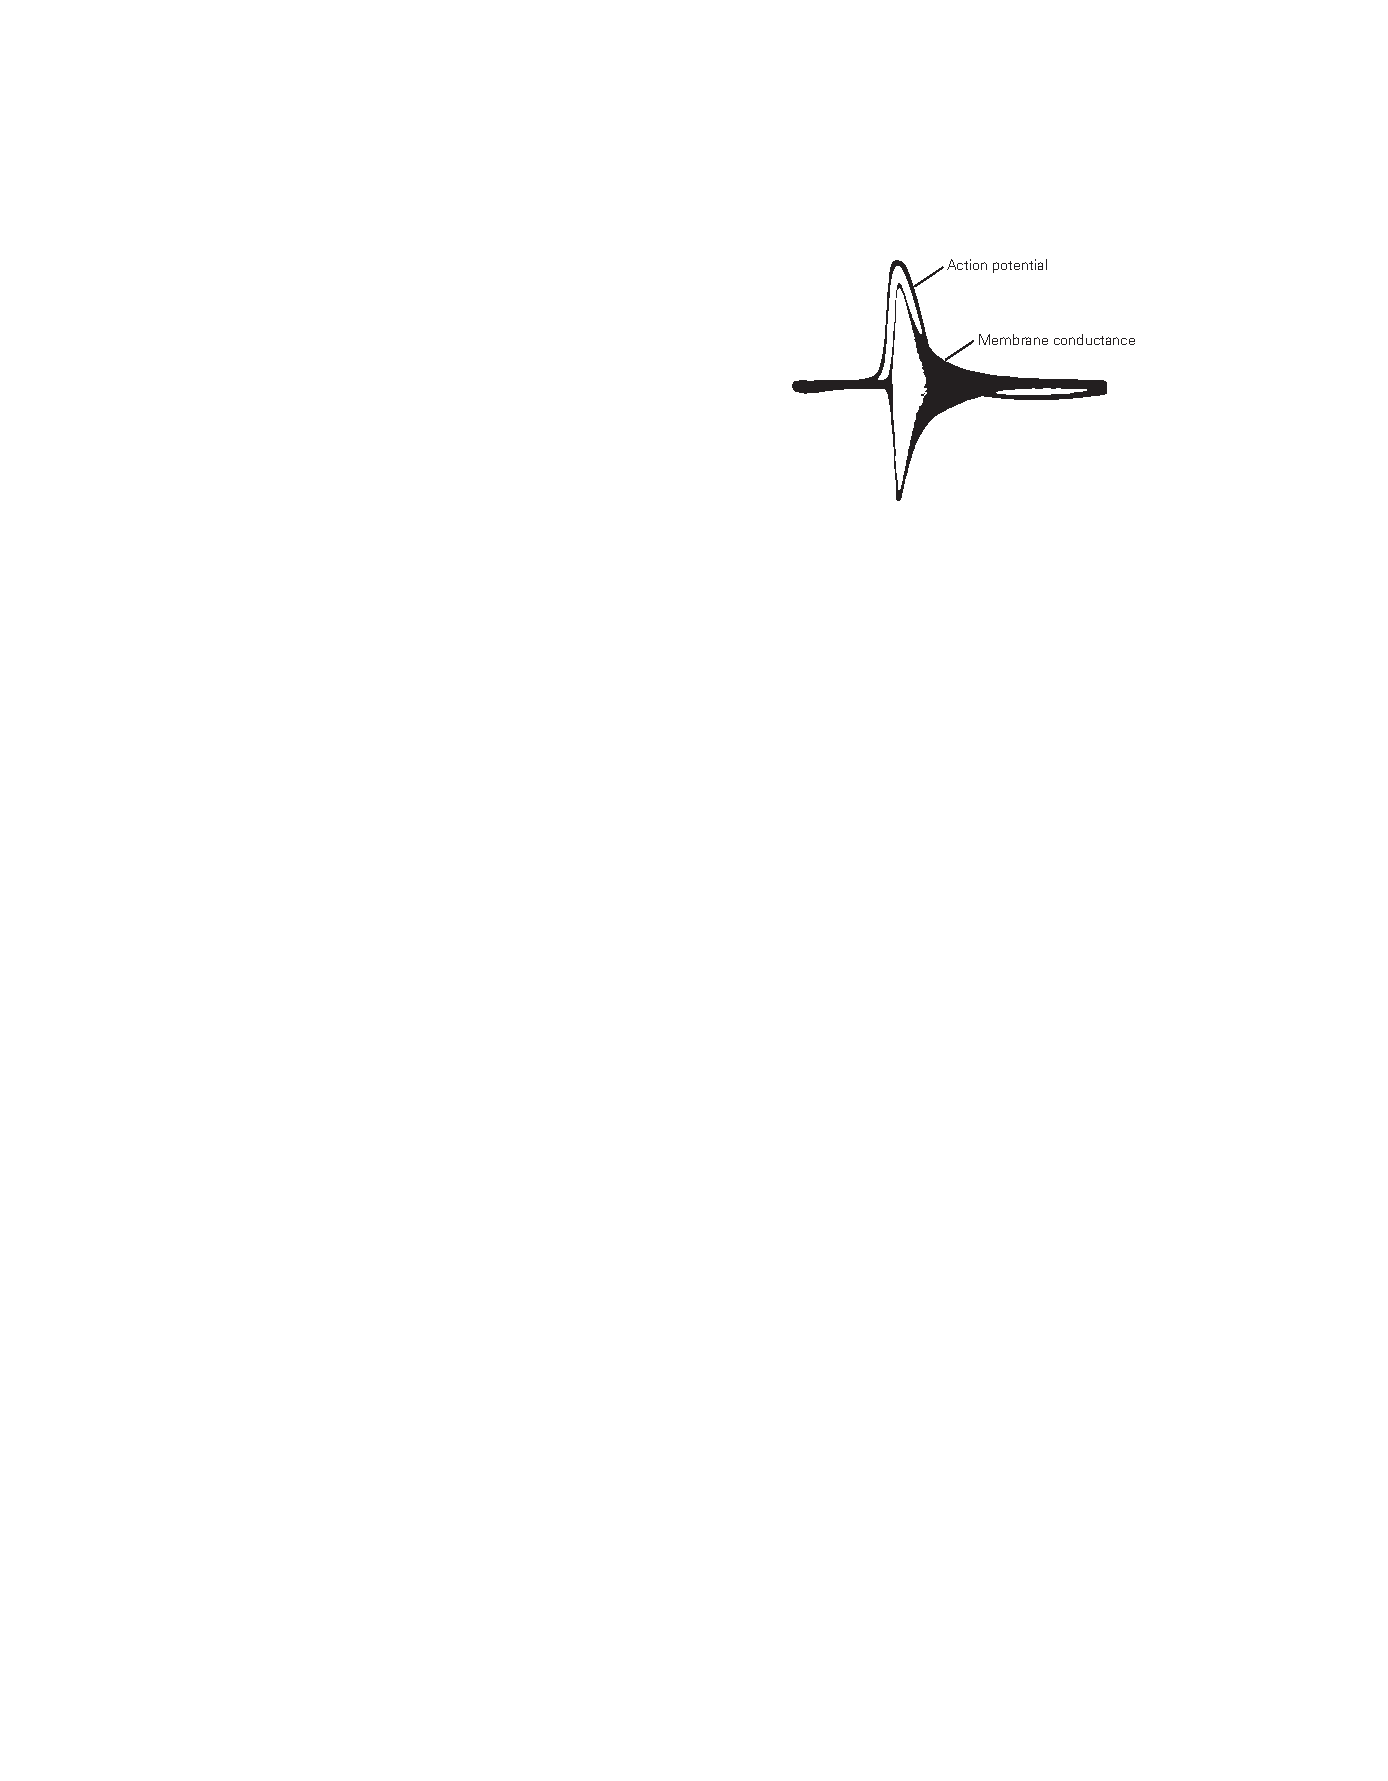
\includegraphics[width=0.5\linewidth]{chap10/fig_10_1}
	\caption{动作电位是由轴突膜离子电导的增加引起的。 肯尼思·科尔 (Kenneth Cole) 和霍华德·柯蒂斯 (Howard Curtis) 于 1939 年进行的一项实验的历史记录显示了动作电位的示波器记录叠加在轴突膜电导的同步记录上。}
	\label{fig:10_1}
\end{figure}


Hodgkin 和 Katz 通过证明当外部 Na+ 浓度降低时动作电位的振幅降低,从而表明 Na+ 流入是动作电位上升阶段的原因,从而提供了对该问题的关键见解。
他们提出,细胞去极化超过动作电位阈值会导致细胞膜的 Na+ 电导短暂增加,在此期间 Na+ 电导压倒在静止细胞中占主导地位的 K+ 电导,从而将膜电位推向 ENa。 
他们的数据还表明,动作电位的下降阶段是由后来的 K+ 渗透性增加引起的。



\subsection{使用电压钳记录通过电压门控通道的钠和钾电流}

Hodgkin 和 Katz 的这一见解提出了一个进一步的问题。
什么机制负责调节膜的 Na+ 和 K+ 渗透性的变化?
Hodgkin 和 Andrew Huxley 推断 Na+ 和 K+ 渗透率直接受膜电压调节。
为了验证这一假设,他们系统地改变了乌贼巨型轴突的膜电位,并测量了由此产生的电压门控 Na+ 和 K+ 通道电导的变化。
为此,他们使用了一种新设备,即肯尼斯·科尔 (Kenneth Cole) 开发的电压钳。


在电压钳技术问世之前,测量 Na+ 和 K+ 电导作为膜电位函数的尝试受到膜电位和 Na+ 和 K+ 通道门控的强相互依赖性的限制。
例如,如果膜去极化到足以打开一些电压门控 Na+ 通道,则通过这些通道流入的 Na+ 会导致进一步去极化。 
额外的去极化导致更多的 Na+ 通道打开,从而诱导更多的内向 Na+ 电流:


这种正反馈循环将膜电位驱动到动作电位的峰值,从而无法达到稳定的膜电位。


电压钳中断了膜电位与电压门控离子通道开闭之间的相互作用。
它通过在轴突中加入或抽取与通过电压门控膜通道的电流相等的电流来实现。
通过这种方式,电压钳可以防止膜电位发生变化。
因此,为保持膜电位恒定而必须由电压钳产生的电流量可直接测量通过电压门控通道的电流(方框 10-1)。
使用电压钳技术,Hodgkin 和 Huxley 能够完整地描述动作电位背后的离子机制。


电压钳的优点之一是它可以轻松地分别分析膜电流的离子和电容分量。
如第~\ref{chap:chap9}~章所述,膜电位 Vm 与膜电容 Cm 上的电荷 Qm 成正比。
当 Vm 不变时,Qm 恒定,没有电容电流 (ΔQm/Δt) 流动。
电容电流仅在 Vm 变化时流动。
因此,当膜电位响应命令的去极化步骤而变化时,电容电流仅在步骤的开始和结束时流动。
由于电容电流基本上是瞬时的,因此可以单独分析随后流经电压门控通道的离子电流。


这些离子电流的测量可用于计算由 Na+ 和 K+ 通道的打开和关闭引起的膜电导变化的电压和时间依赖性。
此信息提供了对这两种类型渠道的属性的深入了解。


典型的电压钳实验从将膜电位钳制在其静止值开始。
当应用一个小的 (10 mV) 去极化步骤时,一个非常短暂的外向电流会瞬间使膜电容放电 10 mV 去极化所需的量。
该电容电流 (Ic) 之后是较小的外向电流,该电流在电压阶跃期间持续存在。
这种稳定的离子电流流过膜的非门控静息离子通道,我们在这里将其称为泄漏通道(见方框 9-2)。
通过这些通道的电流称为漏电流 Il,这些通道的总电导称为漏电导 (gl)。
在该步骤结束时,一个短暂的内向电容电流将膜重新极化到其初始电压,并且总膜电流返回到零(图~\ref{fig:10_3}A)。


\begin{figure}[htbp]
	\centering
	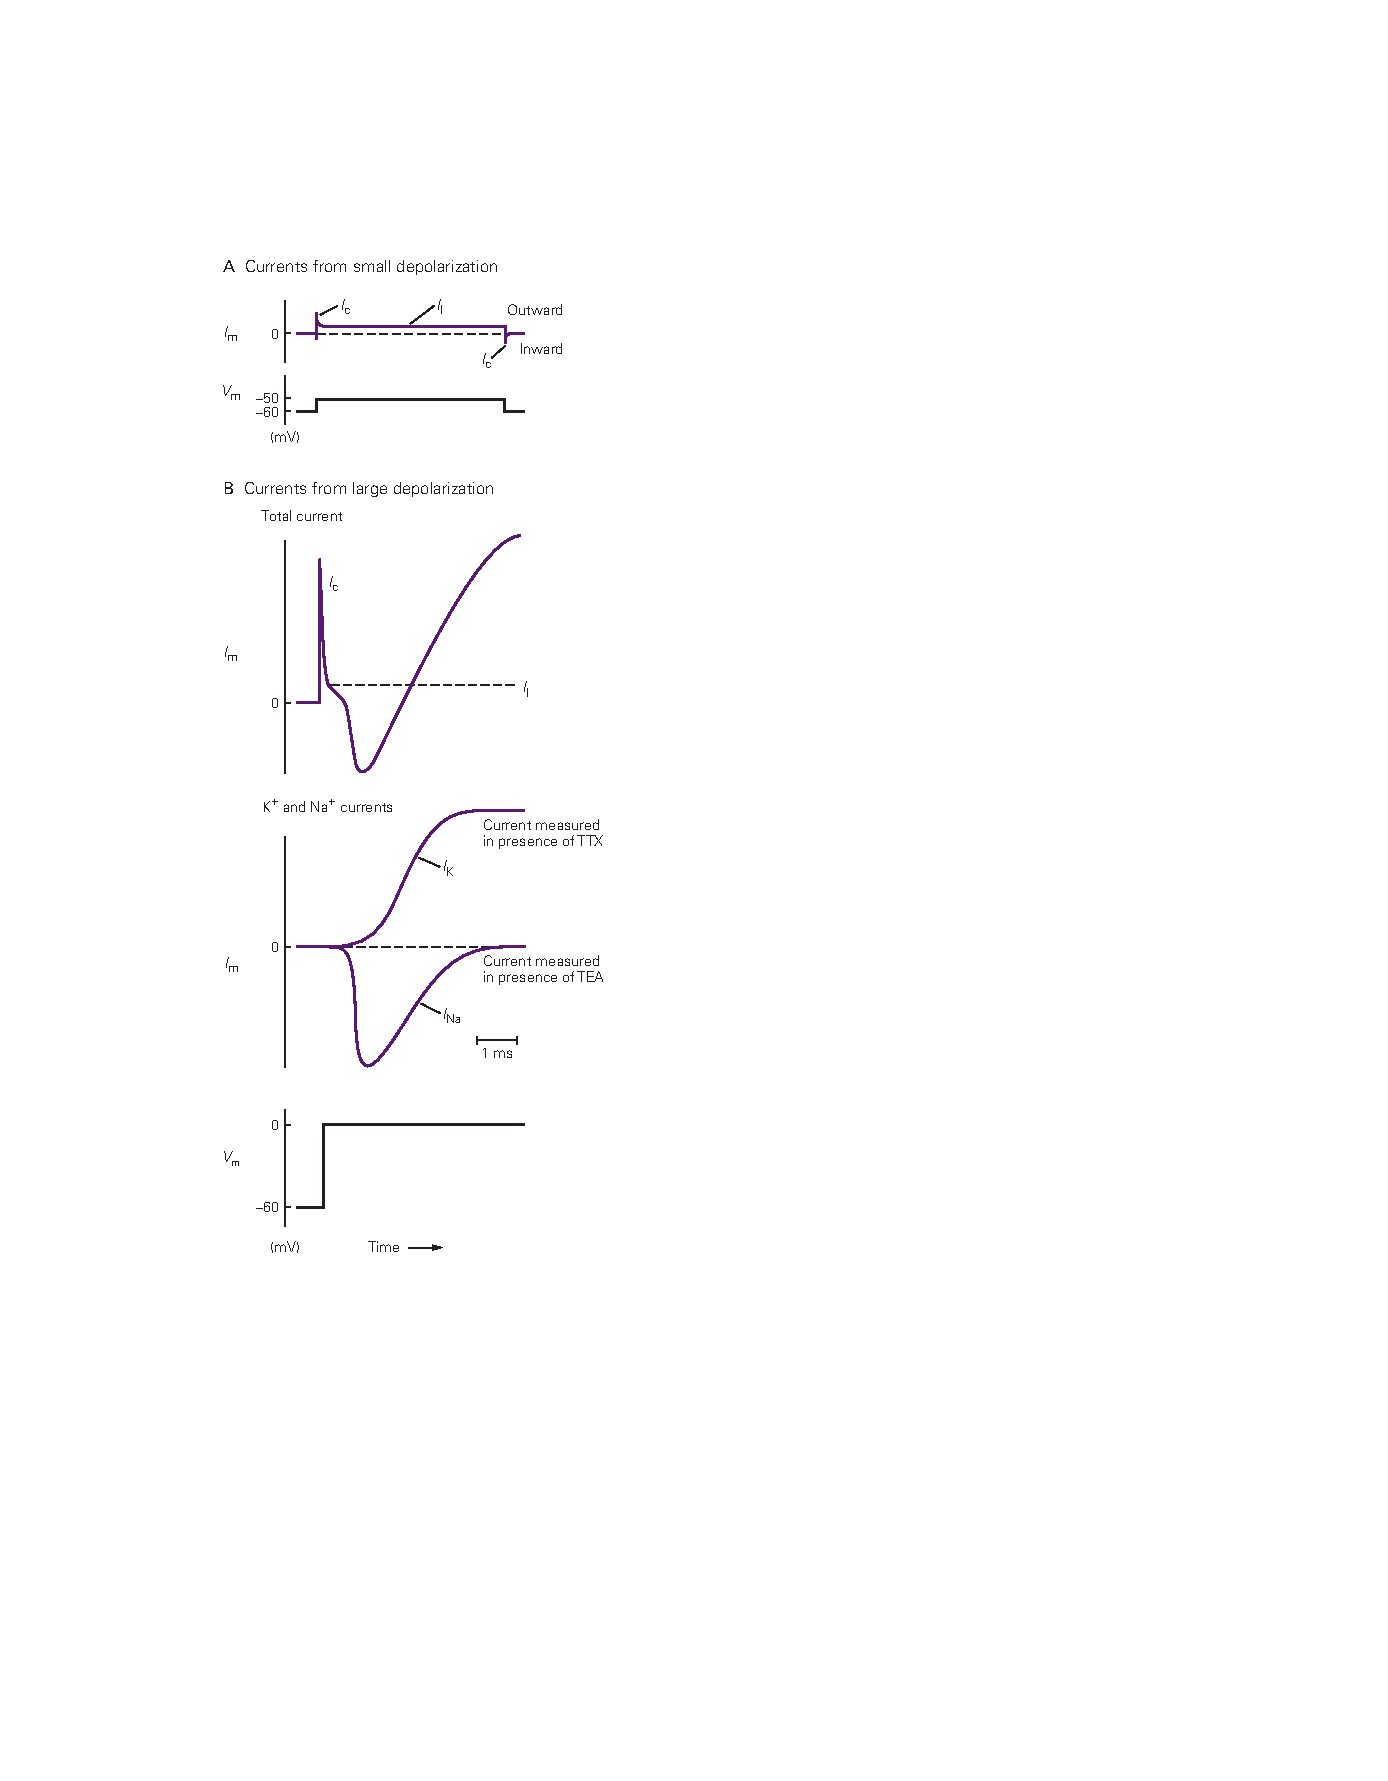
\includegraphics[width=0.4\linewidth]{chap10/fig_10_3}
	\caption{电压钳实验演示了电压门控钠通道和钾通道的顺序激活。 A. 小的去极化 (10 mV) 会引发电容电流和漏电流(分别为 Ic 和 Il),它们是总膜电流 (Im) 的组成部分。 B. 较大的去极化 (60 mV) 会导致较大的电容电流和漏电流,以及随时间变化的内向离子电流和随时间变化的外向离子电流。 顶部:响应去极化的总(净)电流。 中间:单独的 Na+ 和 K+ 电流。 在存在阻断 Na+ 电流的河豚毒素 (TTX) 或存在阻断 K+ 电流的四乙铵 (TEA) 的情况下使细胞去极化,显示减去后的纯 K+ 和 Na+ 电流(分别为 IK 和 INa) Ic 和 Il。 底部:电压阶跃。}
	\label{fig:10_3}
\end{figure}


如果命令大的去极化步骤,则当前记录会更复杂。
电容电流和漏电流的幅度都会增加。
此外,在电容电流结束和泄漏电流开始后不久,会产生一个内向(负)电流;
它在几毫秒内达到峰值,下降,然后让位于外向电流。
该外向电流达到一个平台,该平台在电压阶跃期间保持不变(图 10–3B)。


对这些结果的简单解释是,去极化电压阶跃依次打开两种类型的电压门控通道,每种通道对不同的离子种类具有选择性。
一种类型的通道传导产生快速上升的内向电流的离子,而另一种类型的通道传导产生更缓慢上升的外向电流的离子。
因为这两个方向相反的电流在时间上部分重叠,所以分析电压钳实验最困难的任务是确定它们各自的时间进程。


霍奇金和赫胥黎通过改变沐浴液中的离子实现了这种分离。
通过用更大的非渗透性阳离子(胆碱·H+)代替 Na+,他们消除了内向的 Na+ 电流。
后来,由于发现了选择性阻断不同类别电压门控通道的药物或毒素,分离内向电流和外向电流的任务变得更加容易。
河豚毒素是一种来自太平洋河豚的毒药,在纳摩尔浓度范围内具有非常高的效力,可阻断电压门控 Na+ 通道。
(从作为日本生鱼片美味河豚食用的河豚鱼中,如果处理不当,摄入几毫克河豚毒素就可能致命。)阳离子四乙基铵 (TEA) 会特异性阻断一些电压门控 K+ 通道。


当 TEA 应用于轴突以阻断 K+ 通道时,总膜电流 (Im) 由 Ic、Il 和 INa 组成。
漏电导gl是常数; 它不随 Vm 或时间而变化。
因此,可以很容易地计算出泄漏电流 Il 并从 Im 中减去,剩下 INa 和 Ic。
由于 Ic 仅在脉冲的开始和结束时短暂出现,因此通过目视检查很容易将其分离,显示出纯 INa。
同样,当 Na+ 通道被河豚毒素阻断时,可以测量 IK(图 10–3B)。


通过使膜跨过各种电位,Hodgkin 和 Huxley 能够测量动作电位整个电压范围内的 Na+ 和 K+ 电流(图 ~\ref{fig:10_4})。
他们发现 Na+ 和 K+ 电流随着膜电位的梯度函数而变化。
随着膜电压变得更正,向外的 K+ 电流变得更大。
在一定程度上,内向 Na+ 电流也随着去极化的增加而变大。
然而,随着电压变得越来越正,Na+ 电流的幅度最终会下降。
当膜电位为 +55 mV 时,Na+ 电流为零。
正至 +55 mV,Na+ 电流反转方向并向外。


\begin{figure}[htbp]
	\centering
	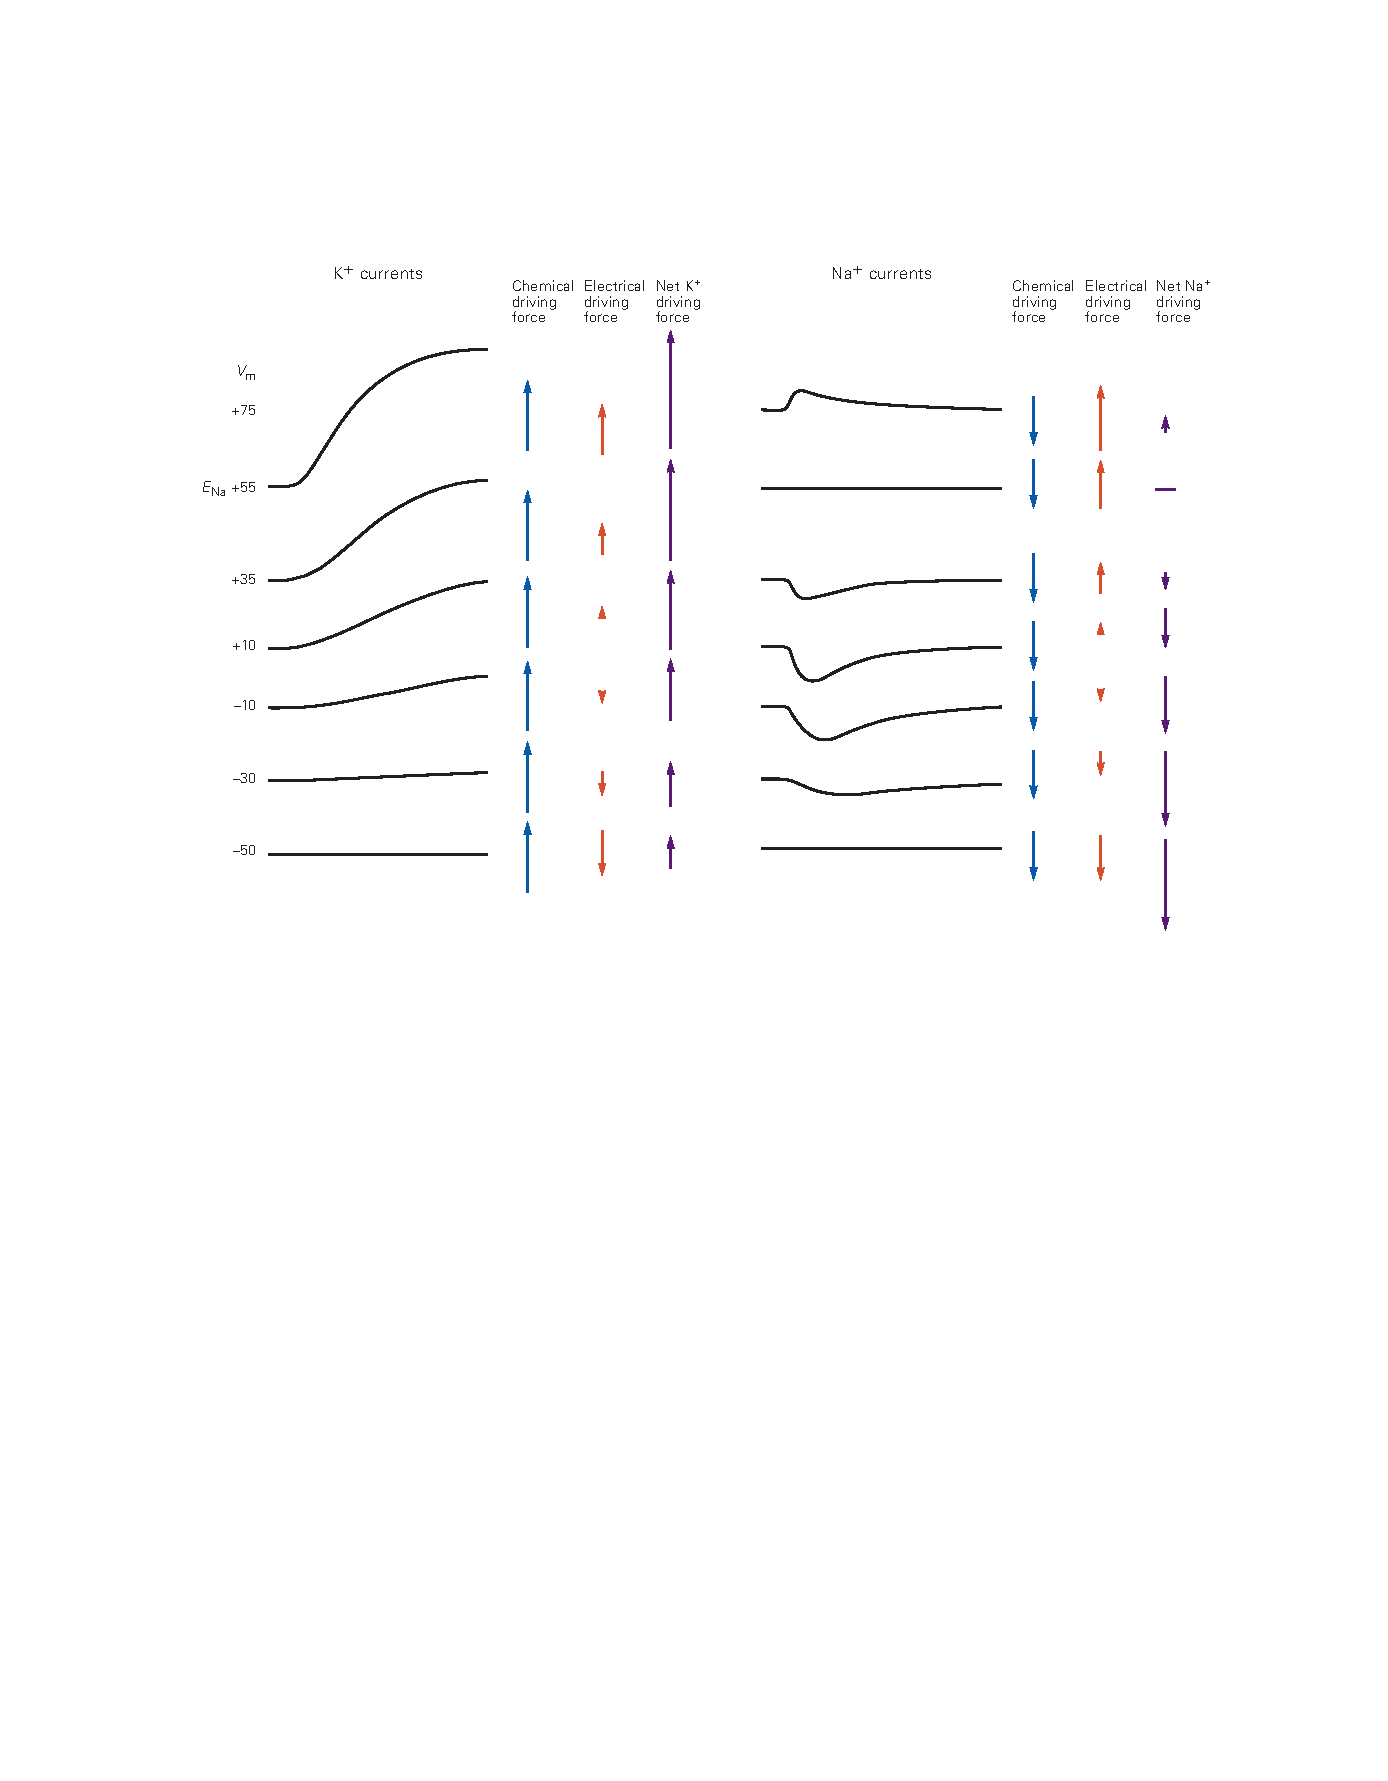
\includegraphics[width=0.8\linewidth]{chap10/fig_10_4}
	\caption{钠和钾膜电流的大小和极性随膜去极化的幅度而变化。 左:随着渐进去极化,电压钳位膜 K+ 电流单调增加,因为 gK 和 (Vm – EK),K+ 的驱动力,随着去极化的增加而增加。 去极化期间的电压显示在左侧。 K+ 上的化学 (EK) 和电驱动力的方向和大小,以及净驱动力,由每条迹线右侧的箭头给出。 (向上箭头 = 向外力;向下箭头 = 向内力。)右图:起初,由于 gNa 的增加,Na+ 电流变得越来越向内,去极化也越来越大。 然而,当膜电位接近 ENa (+55 mV) 时,由于内向驱动力 (Vm – ENa) 的减少,内向 Na+ 电流的幅度开始减小。 最终,当膜电位达到 ENa 时,INa 变为零。 在对 ENa 正去极化时,(Vm – ENa) 的符号反转并且 INa 向外。}
	\label{fig:10_4}
\end{figure}


Hodgkin 和 Huxley 通过一个简单的模型解释了这种行为,其中 Na+ 和 K+ 电流的大小由两个因素决定。
第一个是 Na+ 或 K+ 电导的大小,gNa 或 gK,它反映了在任何时刻打开的 Na+ 或 K+ 通道的数量(第 ~\ref{chap:chap9}~章)。
第二个因素是对 Na+ 离子 (Vm − ENa) 或 K+ 离子 (Vm − EK) 的电化学驱动力。
该模型因此表示为:


根据该模型,INa 和 IK 的幅度随着电压变得更正而变化,因为 gNa 和 gK 增加了。
电导增加是因为 Na+ 和 K+ 通道的打开是电压相关的。
电流也随着电化学驱动力的变化而变化。


INa 和 IK 最初都随着膜变得更积极而增加振幅,因为 gNa 和 gK 随电压急剧增加。
然而,随着膜电位接近 ENa (+55 mV),即使 gNa 很大,INa 也会因为内向驱动力的降低而下降。
也就是说,正膜电压现在反对 Na+ 沿其化学浓度梯度流入。
在 +55 mV 时,化学驱动力和电驱动力处于平衡状态,因此没有净 INa,即使 gNa 相当大。
由于膜对 ENa 呈阳性,因此对 Na+ 的驱动力变为正。 
也就是说,将 Na+ 推出的电驱动力现在大于将 Na+ 拉入的化学驱动力,因此 INa 向外移动。
IK 的行为更简单; EK 非常负 (−75 mV),因此除了 gK 增加外,K+ 的向外驱动力也随着膜变得更正向而变大,从而增加向外的 K+ 电流。



\subsection{电压门控钠和钾电导是根据它们的电流计算的}

Hodgkin 和 Huxley 根据前面的两个方程式,通过将测得的 Na+ 和 K+ 电流除以已知的 Na+ 和 K+ 电化学驱动力,能够计算出 gNa 和 gK。
他们的结果提供了对膜电压如何控制通道开放的直接洞察,因为 gNa 和 gK 的值反映了开放的 Na+ 和 K+ 通道的数量(方框 10-2)。


在不同水平的膜电位下测量 gNa 和 gK 揭示了 Na+ 和 K+ 通道之间的两个功能相似性和两个差异。
两种类型的通道都会响应去极化而打开。
此外,随着去极化大小的增加,两种类型通道的开放程度和速率都会增加。
然而,Na+ 和 K+ 通道的不同之处在于它们打开的速度以及它们对长时间去极化的反应。
在所有去极化水平上,Na+ 通道比 K+ 通道打开得更快(图~\ref{fig:10_6})。 
当去极化持续一段时间后,Na+通道开始关闭,导致内向电流减少。
Na+ 通道在长时间去极化过程中关闭的过程称为失活。


\begin{figure}[htbp]
	\centering
	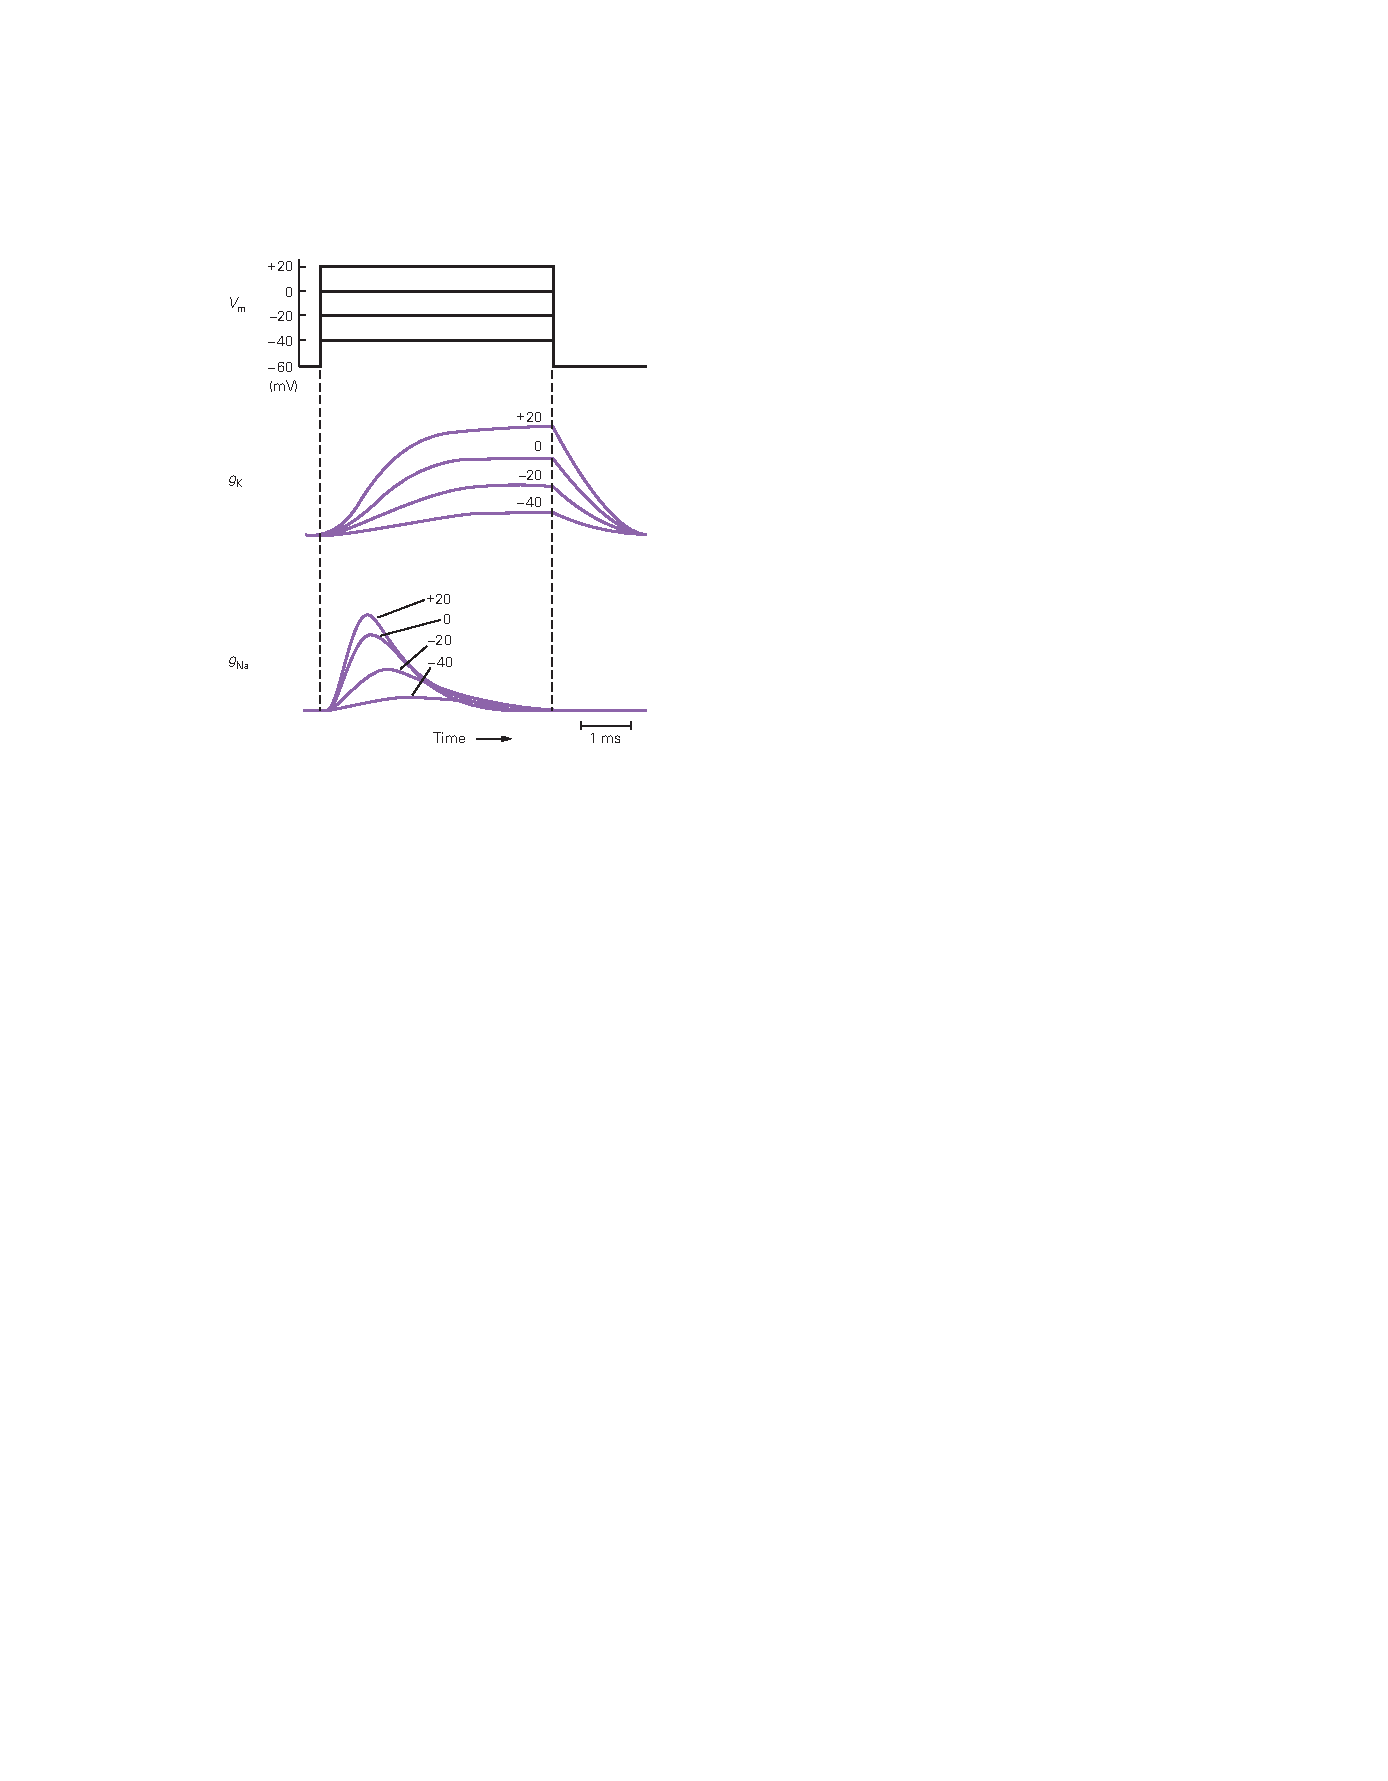
\includegraphics[width=0.5\linewidth]{chap10/fig_10_6}
	\caption{钾和钠离子通道对长时间去极化的反应。 增加去极化引起 K+ 和 Na+ 电导(gNa 和 gK)的分级增加,这反映了数千个电压门控 K+ 和 Na+ 通道的比例开放。 Na+ 通道比 K+ 通道打开得更快。 在维持去极化过程中,由于失活门的关闭,Na+ 通道在打开后关闭。 K+ 通道保持开放状态是因为它们缺乏快速灭活过程。 在非常正的 Vm 下,K+ 和 Na+ 电导接近最大值,因为去极化足以打开几乎所有可用通道。}
	\label{fig:10_6}
\end{figure}


因此,去极化导致 Na+ 通道在三种不同状态(静止、激活或失活)之间切换,这代表 Na+ 通道蛋白的三种不同构象(见图 8-6)。
相反,鱿鱼轴突 K+ 通道不会失活;
只要膜去极化,它们就会保持打开状态,至少对于持续长达数十毫秒的电压钳去极化而言(图~\ref{fig:10_6})。


在失活状态下,Na+ 通道不能通过进一步的膜去极化打开。
这种失活只能通过将膜重新极化到其负静息电位来逆转,于是通道切换到静息状态。
此切换需要一些时间。


去极化对 gNa 的这些可变的、依赖于时间的影响是由 Na+ 通道中两种门控机制的动力学决定的。
每个 Na+ 通道都有一个激活门,当膜处于静息电位时关闭,并通过去极化打开。
失活门在静息电位下打开,并在通道响应去极化打开后关闭。
当两个门都打开时,通道仅在去极化期间的短暂时间内传导 Na+。



\subsection{可以根据钠和钾通道的特性重建动作电位}

Hodgkin 和 Huxley 能够将他们的膜电导测量值与一组经验方程相匹配,这些方程完全描述了 Na+ 和 K+ 电导作为膜电位和时间的函数。
使用这些方程和轴突被动特性的测量值,他们计算了动作电位的形状和传导速度。
值得注意的是,这些方程还提供了对电压门控生物物理基础的深入了解,这些基础在 50 多年后通过 X 射线晶体学阐明了某些电压门控通道的结构时得到了证实。


计算出的动作电位波形与未夹紧轴突中记录的波形几乎完全匹配。
这种紧密一致表明,霍奇金和赫胥黎开发的数学模型准确地描述了负责产生和传播动作电位的通道的特性。
半个多世纪后,霍奇金-赫胥黎模型成为神经科学中最成功的定量模型,如果不是整个生物学的话。


根据该模型,动作电位涉及以下事件序列。
膜的去极化导致 Na+ 通道快速打开(gNa 增加),导致内向 Na+ 电流。
该电流通过使膜电容放电,导致进一步去极化,从而打开更多的 Na+ 通道,导致内向电流进一步增加。 
这种再生过程将膜电位推向 ENa,导致动作电位的上升阶段。
去极化以两种方式限制动作电位的持续时间:
(1) 它逐渐使电压门控 Na+ 通道失活,从而减少 gNa,
(2) 它在一定延迟后打开电压门控 K+ 通道,从而增加 gK。
因此,内向 Na+ 电流之后是外向 K+ 电流,倾向于使膜复极化(图~\ref{fig:10_7})。


\begin{figure}[htbp]
	\centering
	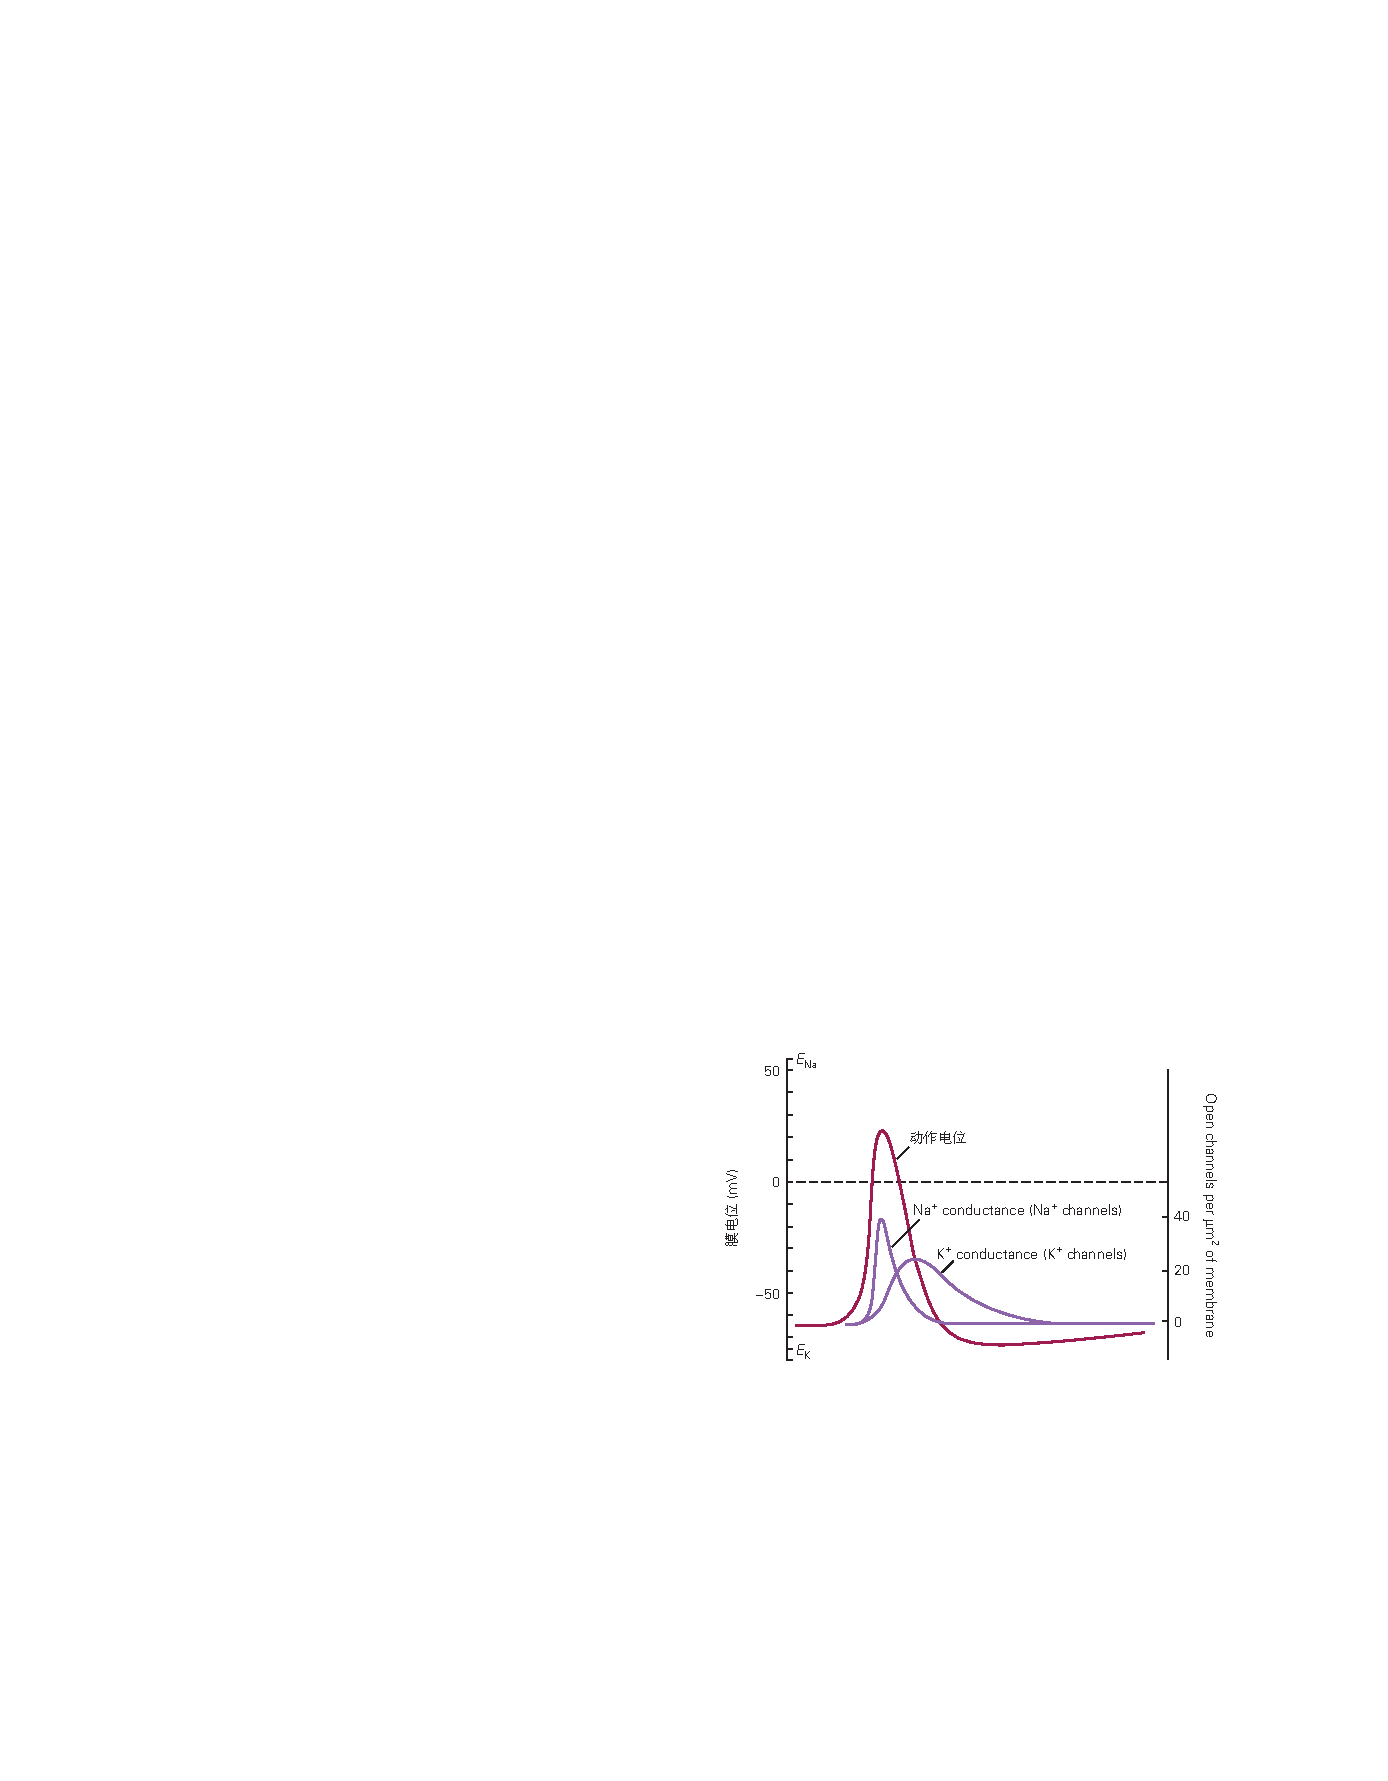
\includegraphics[width=0.5\linewidth]{chap10/fig_10_7}
	\caption{电压门控 Na+ 和 K+ 通道的顺序打开会产生动作电位。 Hodgkin 和 Huxley 的一项伟大成就是将动作电位期间电导的变化分解为可归因于 Na+ 和 K+ 通道开放的独立成分。 动作电位的形状和潜在的电导变化可以根据电压门控 Na+ 和 K+ 通道的特性来计算。 (经许可改编自 Hille 2001。)}
	\label{fig:10_7}
\end{figure}


Hodgkin-Huxley 模型预测的动作电位的两个特征是它的阈值和 allor-none 行为。
毫伏的几分之一可能是亚阈值刺激与产生全尺寸动作电位的刺激之间的差异。
当人们认为 Na+ 电导随着去极化的增加而以严格分级的方式增加时,这种全有或全无的现象似乎令人惊讶(图 ~\ref{fig:10_6})。 
去极化的每次增量都会增加打开的电压门控 Na+ 通道的数量,从而逐渐增加 Na+ 电流。
那么如何才能有一个离散的阈值来产生动作电位呢?


尽管小的亚阈值去极化增加了向内的 INa,但它也通过增加作用于 K+ 和 Cl- 的电化学驱动力增加了两个外向电流 IK 和 Il。
此外,去极化通过逐渐打开更多电压门控 K+ 通道来增强 K+ 电导(图~\ref{fig:10_6})。 
随着向外的 K+ 和漏电流随着去极化而增加,它们倾向于使膜复极化,从而抵抗 Na+ 流入的去极化作用。
然而,由于 Na+ 通道的高电压敏感性和更快速的激活动力学,去极化最终达到向内 INa 的增加超过向外 IK 和 Il 的增加的点。
此时,存在净内向离子电流。
这会产生进一步的去极化,打开更多的 Na+ 通道,使去极化变得再生,快速驱动膜电位 Vm 一直到动作电位的峰值。
净离子电流 (INa + IK + Il) 从外向内变化、在膜电容内部沉积正电荷时的 Vm 特定值是阈值。


神经纤维细胞外刺激的早期实验表明,在动作电位后的短时间内(通常是几毫秒),不可能产生另一个动作电位。 
这个绝对不应期之后是一个可以刺激另一个动作电位的时期,但只能使用比第一次所需的刺激更大的刺激。 
该相对不应期通常持续 5 至 10 毫秒。


Hodgkin-Huxley 分析为不应期背后的两个因素提供了机制解释。
在一个动作电位之后,即使有非常强的刺激,也不可能唤起另一个动作电位,因为 Na+ 通道仍然处于失活状态。 
复极化后,Na+ 通道从失活状态恢复并重新进入静息状态,这一转变需要几毫秒(图~\ref{fig:10_8})。 
相对不应期对应于从失活中部分恢复。


\begin{figure}[htbp]
	\centering
	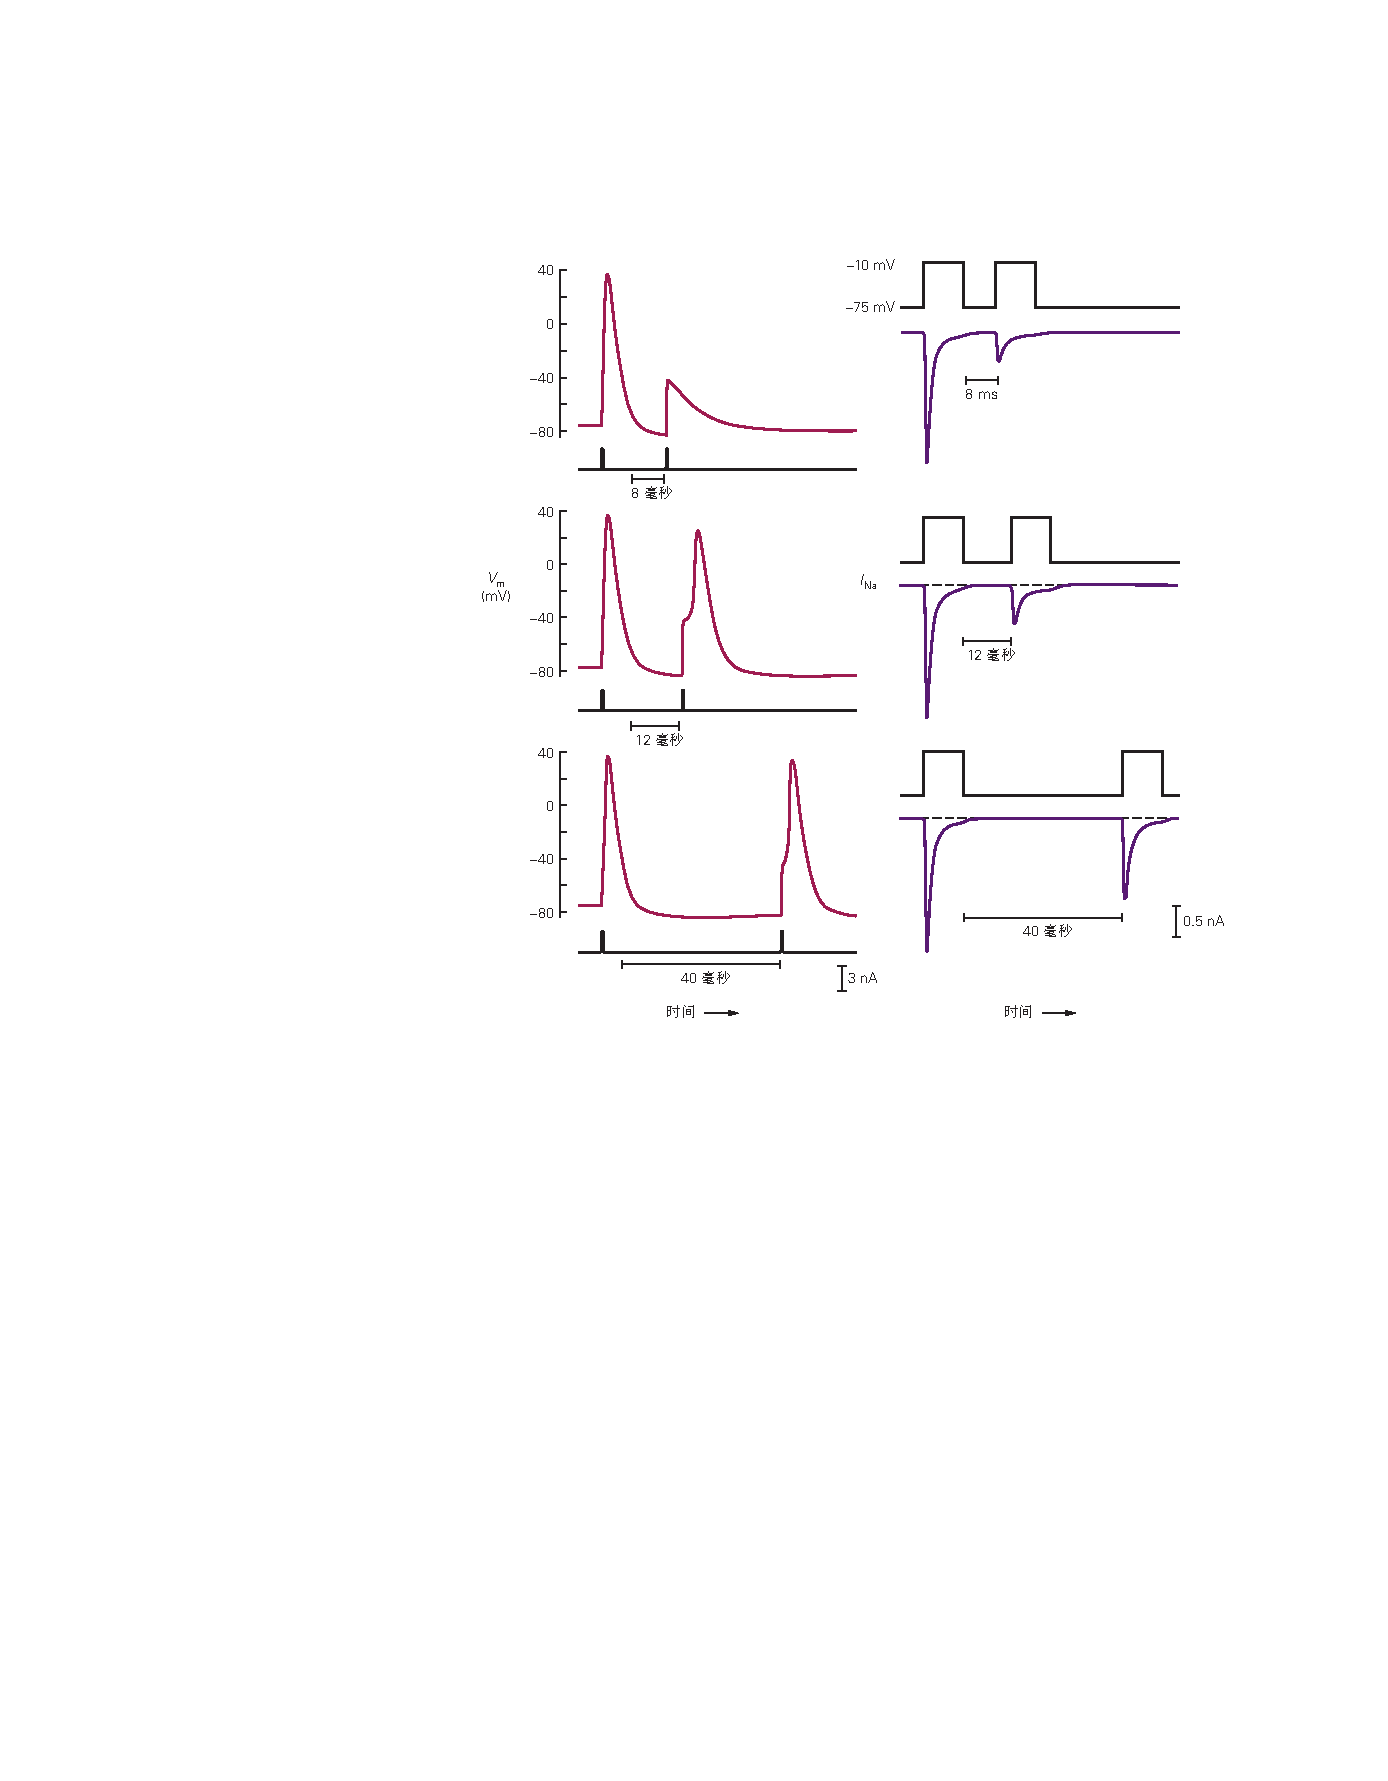
\includegraphics[width=0.7\linewidth]{chap10/fig_10_8}
	\caption{不应期与钠通道从失活中恢复有关。 左图:小鼠背根神经节神经元对两个电流脉冲的电压响应(底部迹线)。 第一个触发动作电位; 第二个触发可变电压响应,具体取决于电流脉冲之间的延迟。 右图:由两个去极化电压脉冲引起的同一个电池在电压钳下记录的钠电流,两个去极化电压脉冲由左侧记录中指示的间隔分开。 在这个神经元中,不应期对应于恢复大约 20\% 的钠通道所需的时间。 (数据来自 Pin Liu 和 Bruce Bean。)}
	\label{fig:10_8}
\end{figure}


相对不应期还受动作电位后 K+ 电导残留增加的影响。 
在动作电位期间打开的所有 K+ 通道都需要几毫秒才能恢复到其关闭状态。
在此期间,当 K+ 电导略微升高时,Vm 比其正常静息值稍微负一些,因为 Vm 接近 EK(图~\ref{fig:10_7},公式 9-4)。 
这种后超极化和 gK 的残余增加有助于在相对不应期期间将 Vm 驱动到阈值所需的去极化电流的增加。




\section{电压门控的机制已从电生理测量中推断出来}

霍奇金和赫胥黎推导出的经验方程非常成功地描述了离子流如何通过 Na+ 和 K+ 通道产生动作电位。
然而,这些方程根据膜电导和电流的变化描述了激发过程。
他们很少谈及响应膜电位变化而激活或失活通道的机制,或关于特定离子的通道选择性。


我们现在知道,Hodgkin 和 Huxley 描述的电压依赖性电导是由以电压和时间依赖性方式打开的离子通道产生的。
来自各种神经和肌肉细胞的膜片钳记录提供了有关产生动作电位的电压依赖性 Na+ 通道特性的详细信息。
单个电压门控 Na+ 通道的记录显示,响应去极化步骤,每个通道以全有或全无的方式打开,传导恒定幅度但持续时间可变的短暂电流脉冲。


每个通道打开都与大约 1 pA 的电流(在接近 −30 mV 的电压下)相关,并且打开状态会因失活而迅速终止。 
每个通道的行为都是随机的,在可变时间后打开并在停用之前保持打开一段可变时间。
如果将响应阶跃去极化的细胞膜中所有通道的开口求和,或者将单个通道对同一去极化的多次试验的开口求和(图 ~\ref{fig:10_9}),则结果是平均电流 与电压钳实验中记录的宏观 Na+ 电流相同的时间过程(参见图 \ref{fig:10_4}B)。


\begin{figure}[htbp]
	\centering
	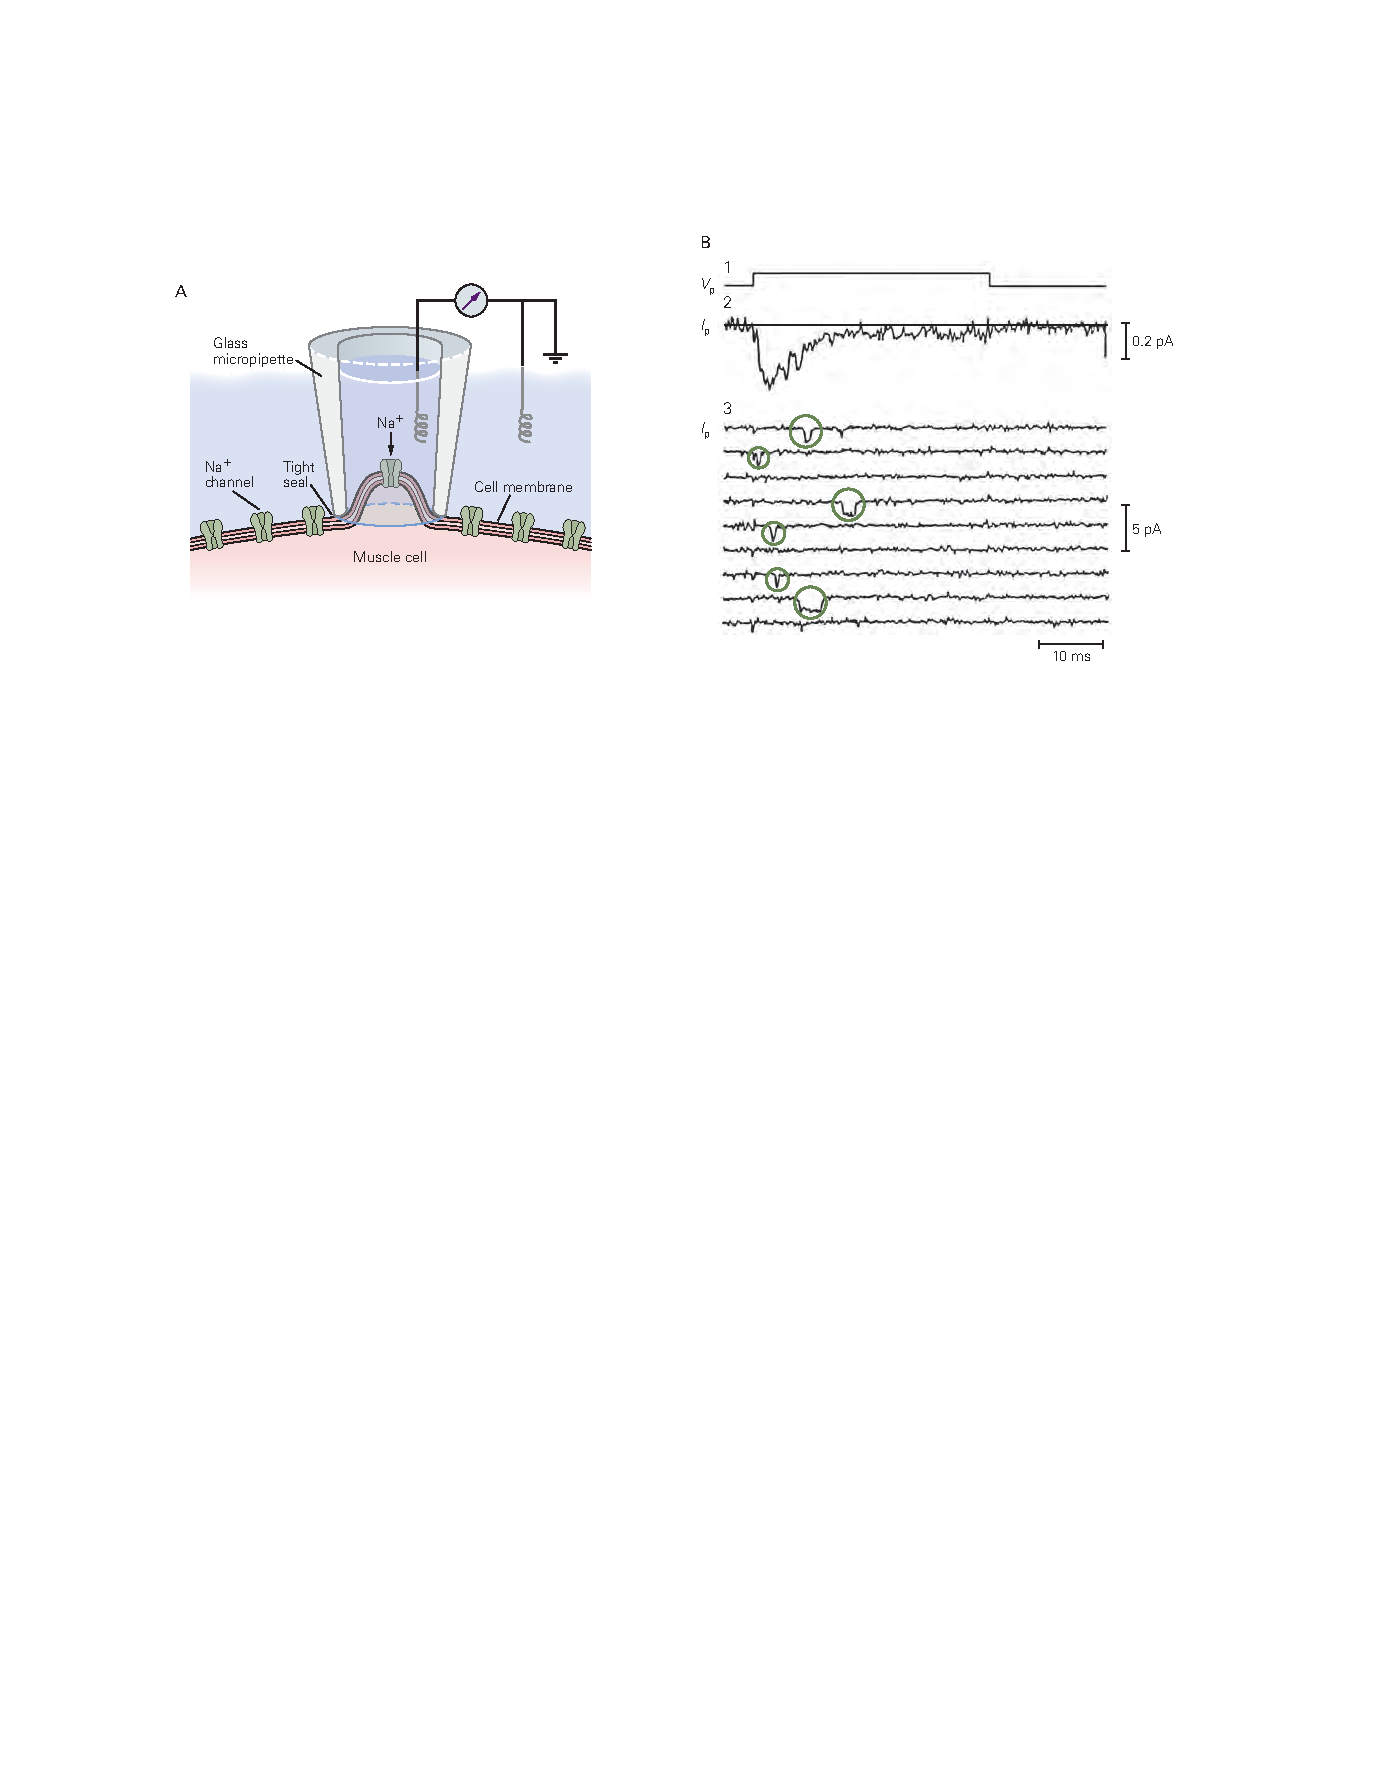
\includegraphics[width=0.5\linewidth]{chap10/fig_10_9}
	\caption{各个电压门控离子通道以全有或全无的方式打开。 A. 一小块包含单个电压门控 Na+ 通道的膜通过贴片电极与细胞的其余部分电隔离。 通过通道进入细胞的 Na+ 电流由连接到贴片电极的监视器记录(见方框 8-1)。 B. 培养的大鼠肌肉细胞中单个 Na+ 通道的记录。 (1) 在隔离的膜片上施加 10 mV 去极化电压阶跃的时间过程(Vp = 膜片上的电位差)。 (2) 在 300 次试验期间通过贴片中 Na+ 通道的内向电流总和(Ip = 通过贴片的电流)。 通过用四乙铵封闭 K+ 通道并以电子方式减去泄漏电流和电容电流来获得迹线。 (3) 300 组中的九个单独试验,显示通道的六个开口(圆圈)。 这些数据表明,传统电压钳记录中记录的总 Na+ 电流(参见图 10–3B)可以通过大量 Na+ 通道的全开或全开的统计性质来解释。 (经许可转载自 Sigworth 和 Neher 1980。)}
	\label{fig:10_9}
\end{figure}


为了解释膜电位的变化如何导致 Na+ 电导的增加,Hodgkin 和 Huxley 从基本的热力学考虑推断出,调节电导的某些膜成分的构象变化必须使带电粒子通过膜电场。 
结果,膜去极化会施加一个力,导致带电粒子移动,从而打开通道。
对于带有带正电的移动粒子的通道,去极化会产生电荷向外移动,这应该先于通道打开。
膜复极化后,电荷会向相反方向移动,从而关闭通道。 
因为移动电荷运动被限制在膜内,所以它是一种电容电流。
预计这种门控电荷运动会产生一个小的外向电流(或门控电流),后来在使用非常灵敏的技术检查膜电流时证实了这一点。
用河豚毒素阻断内向离子电流显示在通道激活期间有一个小的外向电容电流(图~\ref{fig:10_10}A)。 
在后来的实验中,通过将 Na+ 通道的四个 S4 跨膜区域中带正电荷的赖氨酸和精氨酸残基突变为中性残基,该门控电流 (Ig) 逐渐降低。 
因此,门控电流是由 S4 区带正电的残基通过膜电场向外移动产生的(第~\ref{chap:chap8}~章)。 
电压门控 K+ 和 Ca2+ 通道在通道打开期间也会产生门控电流。


\begin{figure}[htbp]
	\centering
	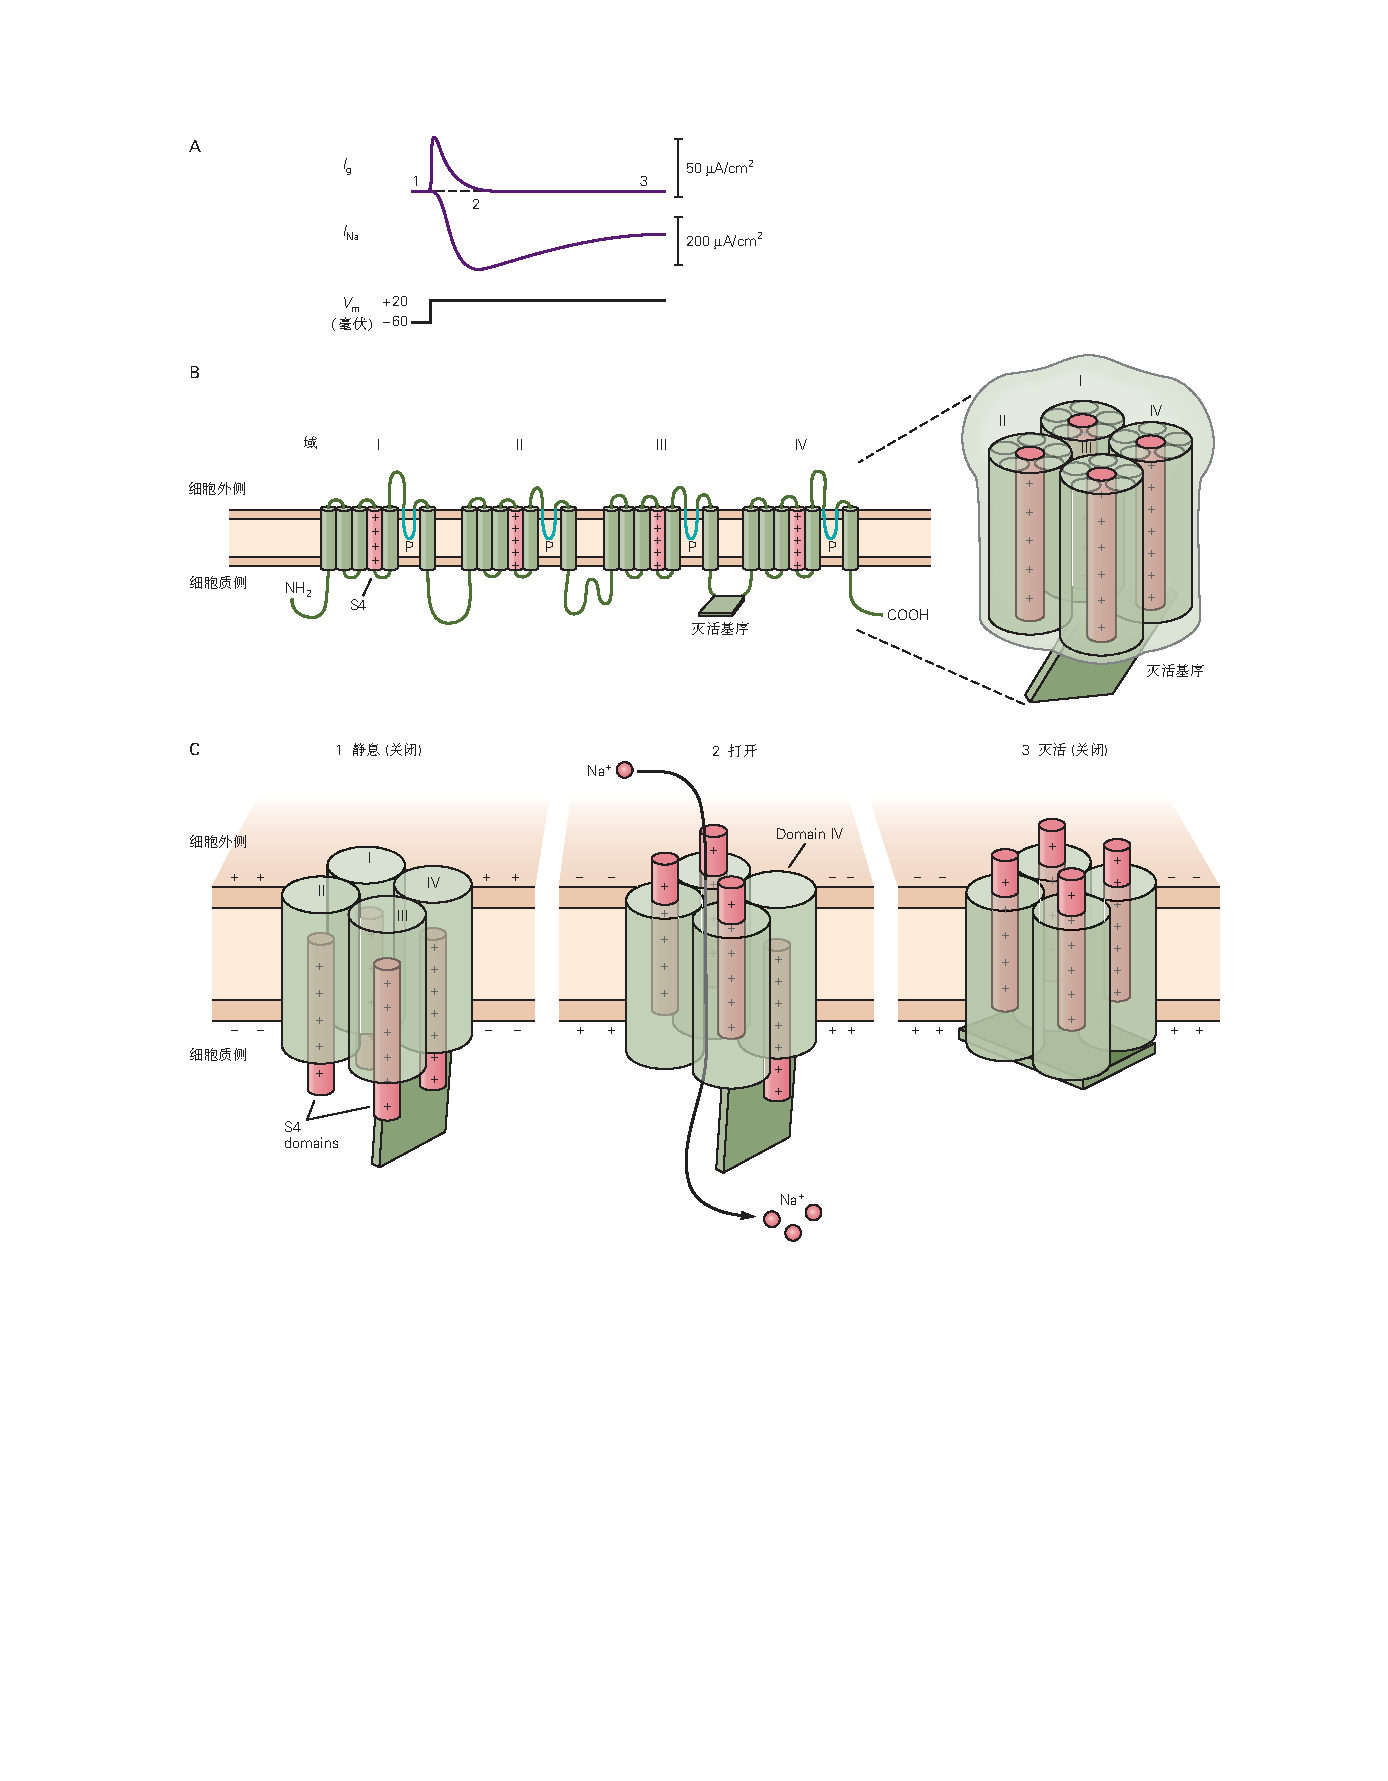
\includegraphics[width=0.8\linewidth]{chap10/fig_10_10}
	\caption{钠通道的打开和关闭与电荷的重新分配有关。 A. 当膜去极化时,Na+ 电流 (INa) 被激活然后失活。 Na+ 电流的激活之前是一个短暂的电容性门控电流 (Ig),反映了正电荷在 Na+ 通道壁内向外移动。 为了检测这个小的门控电流,有必要阻止离子电流流过 Na+ 和 K+ 通道,并减去使脂质双层去极化的电容电流。 (经许可改编自 Armstrong 和 Gilly 1979。)B. 哺乳动物钠通道 α-亚基的二级结构显示门控电荷的位置。 钠通道 α 亚基是由四个重复结构域组成的单一多肽,每个结构域包含六个跨膜区域。 每个结构域的第四个跨膜区(S4 区)包含带正电的精氨酸和赖氨酸残基,它们形成通道的门控电荷。 (经许可改编自 Ahern 等人,2016 年。许可通过 Copyright Clearance Center, Inc. 传达。)C. 图表描绘了当通道处于静止、打开和 灭活。 红色圆柱体代表包含正门控电荷的 S4 区域。 细胞膜从静止状态去极化导致门控电荷向外移动。 结构域 I、II 和 III 的 S4 区域向外运动与激活相关 (1-2),而结构域 IV 的 S4 区域较慢的运动与失活相关 (2-3)。 域 IV 的 S4 区域的移动允许域 III 和 IV 之间的细胞内环(描绘为绿色矩形)结合到孔内部 S6 螺旋附近的停靠位点,变构地稳定失活的闭合状态。 (改编自 Ahern 等人,2016 年。)}
	\label{fig:10_10}
\end{figure}



最近的实验表明,Na+ 通道的四个 S4 跨膜区域随着不同的时间进程移动。 
前三个结构域(DI、DII、DIII)的 S4 区域首先发生运动,并与通道激活相关。 
域 IV 的 S4 区域的运动发生得更慢并且与失活有关。 
Na+ 通道的失活可能涉及一系列构象变化,由此结构域 IV 的 S4 区域向外移动使得连接结构域 III 和 IV 的细胞质接头能够结合到靠近成孔 S6 螺旋细胞内末端的结合位点,从而稳定 孔的非导电失活状态(图 10–10B、C)。


通过门控电荷控制通道激活导致电压依赖性通道的特征:电导变化发生在相对较窄的 Vm 范围内,具有较大去极化的饱和值。
当在宽 Vm 范围内测量峰值 INa 然后转换为电导时,如图~\ref{fig:10_6}~所示,峰值电导的电压依赖性呈 S 形(图 \ref{fig:10_11})。
电压依赖性钠电导的激活开始于约 -50 mV(接近动作电位触发的阈值),达到接近 -25 mV 的中点,并在约 0 mV 时饱和。 
当整个 Na+ 通道群的 S4 区域移动到激活构象时,就会发生电导饱和。


\begin{figure}[htbp]
	\centering
	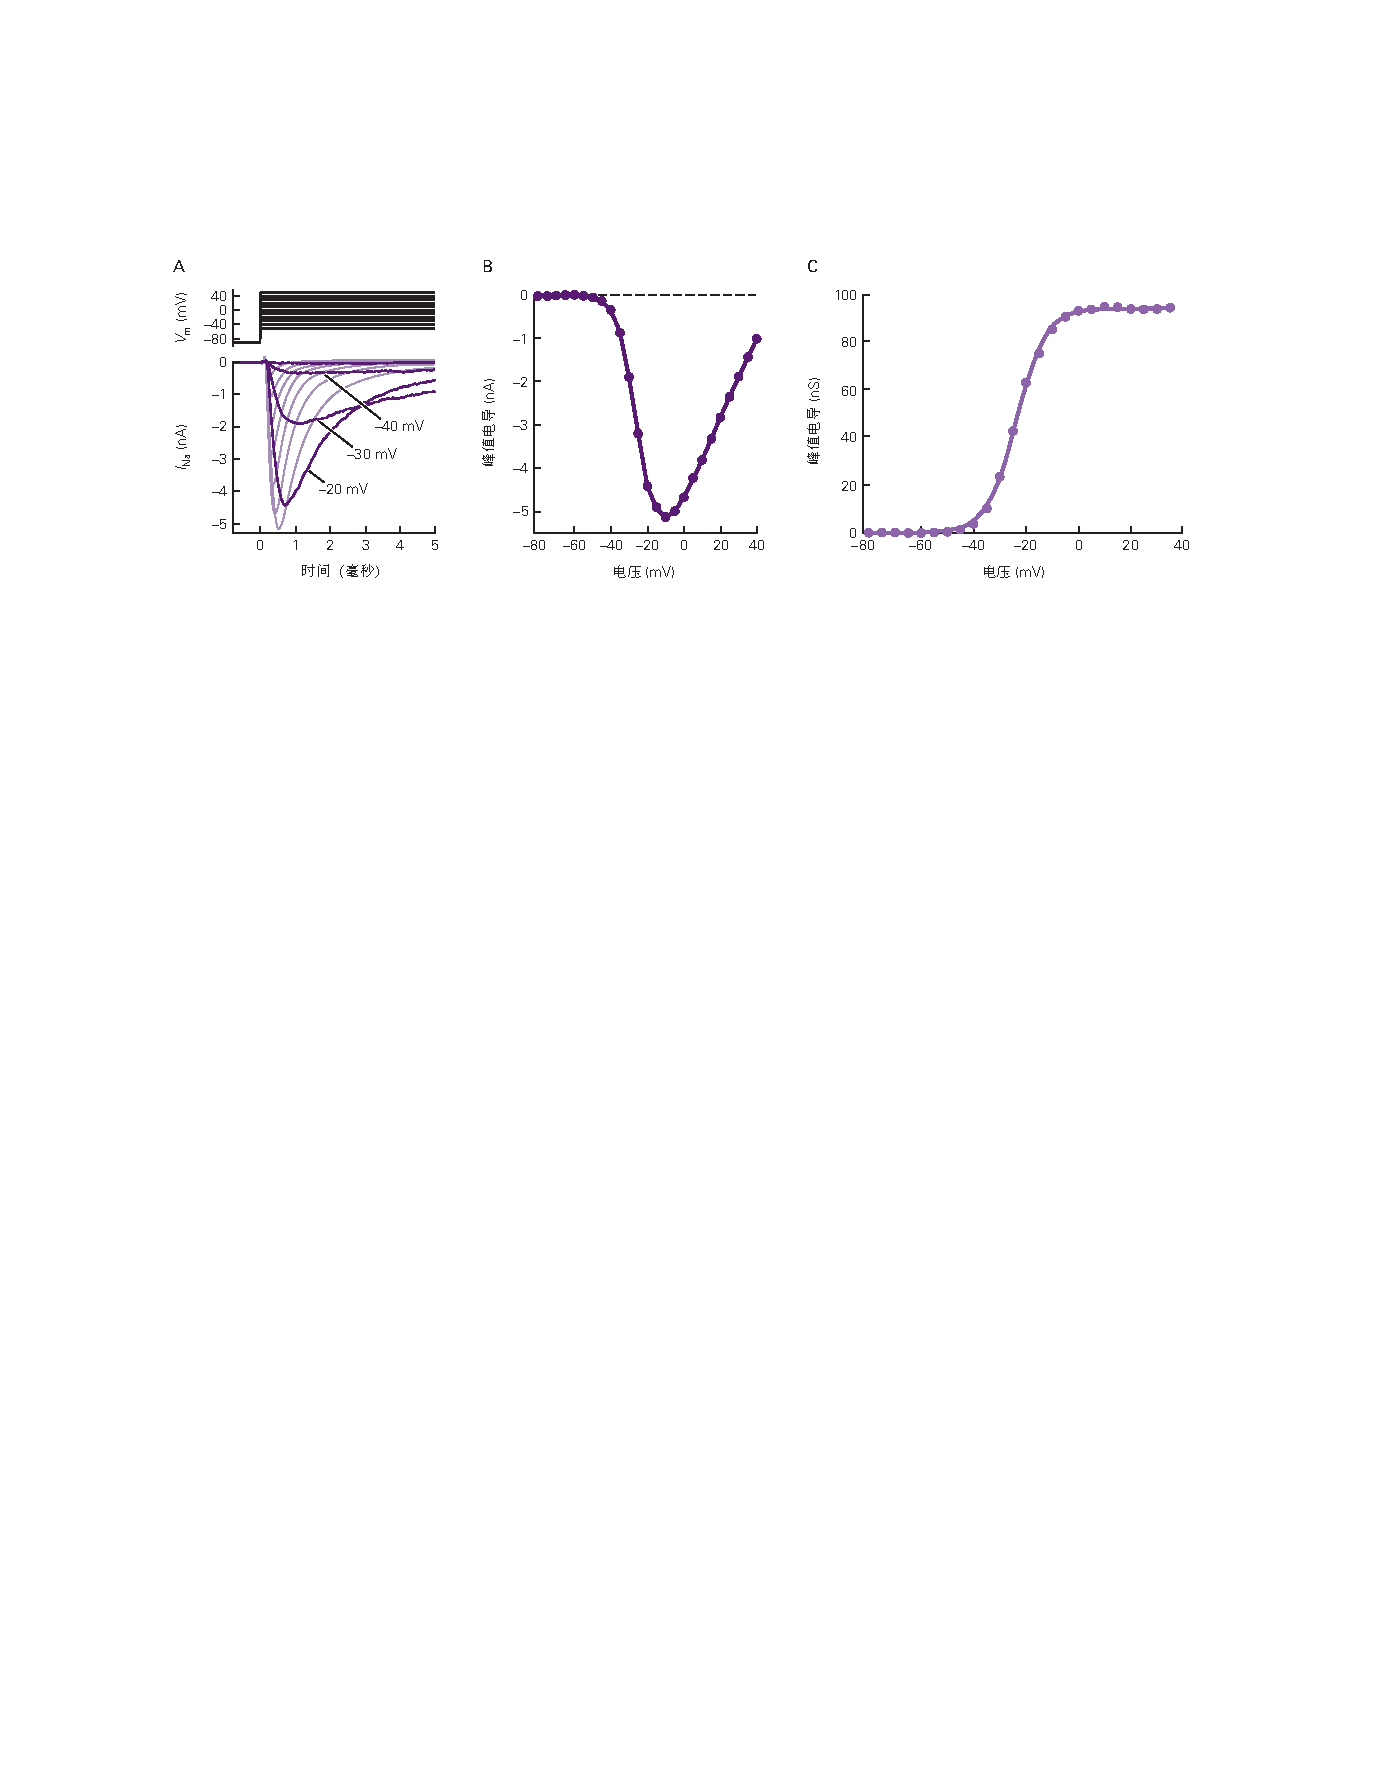
\includegraphics[width=0.9\linewidth]{chap10/fig_10_11}
	\caption{钠通道激活的电压依赖性由门控电荷的数量决定。 A. 在分离的海马锥体神经元中进行电压门控 Na+ 电流的全细胞膜片钳记录。 通过阻断通过 K+ 和 Ca2+ 通道的电流,然后减去阻断 Na+ 电流后剩余的电容电流和漏电流,从而隔离钠通道电流。 B. 峰值 Na+ 电流的电流-电压曲线。 C. 峰值 Na+ 电导与膜电位。 如方框 10-2 所示,根据峰值电流计算一系列去极化电压阶跃导致的峰值 gNa 增加。 实验数据点符合玻尔兹曼关系,形式为 gNa /gNa(max) = 1/ [1 + exp − (Vm − Vh)/k],其中 Vh = −24 mV 是激活曲线的中点, k = 5.5 是“斜率因子”,单位为 mV,gNa(max) 是正电压下的最大钠电导。 打开通道必须移动的门控电荷数量越多,斜率因子就越小。 大多数电压门控通道的电压依赖性可以通过类似的玻尔兹曼曲线来拟合。 (数据来自 Indira M. Raman。)}
	\label{fig:10_11}
\end{figure}


电导与电压的关系可以通过玻尔兹曼函数近似拟合,玻尔兹曼函数是统计力学中的一个方程,描述了分子群的分布,这些分子可以以具有不同势能的不同状态存在。
在 Na+ 通道的情况下,由于 S4 区域门控电荷穿过膜的电场时所做的功,通道在闭合和打开状态之间移动,势能不同(图 10–10C)。
拟合玻尔兹曼曲线的两个参数,中点和斜率因子,提供了通道打开的电压依赖性的方便表征。
如果更多的门控电荷随着通道在关闭和打开状态之间转换而移动,则曲线会更陡峭。
许多其他类型的电压依赖性通道的激活和失活的电压依赖性也可以通过具有特征中点和斜率的玻尔兹曼曲线来近似。


\section{电压门控钠通道根据离子的大小、电荷和水合能量选择钠}

在第~\ref{chap:chap8}~章中,我们看到了 K+ 通道孔的结构如何解释这些通道如何能够选择 K+ 而不是 Na+ 离子。
K+ 通道选择性过滤器的窄直径(约 0.3 nm)要求 K+ 或 Na+ 离子必须排出几乎所有的水合水才能进入通道,这在能量上是不利的事件。


K+ 离子脱水的能量成本通过其与 K+ 通道选择性过滤器的四个亚基的肽主链贡献的电负性羰基氧原子笼的紧密相互作用得到很好的补偿。
由于其半径较小,Na+ 离子比 K+ 离子具有更高的局部电场,因此与水合水的相互作用比 K+ 更强。
另一方面,Na+ 离子的小直径排除了与选择性过滤器中羰基氧原子笼的紧密相互作用;
Na+ 离子脱水所产生的高能量成本使其无法进入通道。


那么 Na+ 通道的选择性过滤器如何选择 Na+ 而不是 K+ 离子?
Bertil Hille 通过测量通道对一系列有机和无机阳离子的相对渗透性,推导出了 Na+ 通道选择性机制的模型。
正如我们在第~\ref{chap:chap8}~章中了解到的,通道的行为就好像它包含一个选择性过滤器或识别位点,它部分地根据大小进行选择,因此充当分子筛(见图 ~\ref{fig:8_1})。
根据可以轻易渗透通道的最大有机阳离子的尺寸和氢键特性,Hille 推断出选择性过滤器的矩形尺寸为 0.3 × 0.5 nm。
这个横截面刚好足以容纳一个 Na+ 离子接触一个水分子(见图 8-1)。
因为与一个水分子接触的 K+ 离子比选择性过滤器的尺寸大,所以它不容易渗透。


根据 Hille 的模型,带负电荷的谷氨酸或天冬氨酸残基的羧酸基团位于孔的外口,通过吸引阳离子和排斥阴离子来执行选择过程的第一步。
负羧酸基团以及排列在孔隙中的其他氧原子可以替代水合水,但这种替代的有效性程度因离子种类而异。
羧酸的负电荷能够与较小的 Na+ 离子形成比与较大的 K+ 离子更强的库仑相互作用。
由于 Na+ 通道足够大以容纳与多个水分子接触的阳离子,因此脱水的能量消耗不如 K+ 通道大。
由于这两个特征,Na+ 通道能够选择 Na+ 而不是 K+,但并不完美,PNa/PK ~ 12/1。
通过 X 射线晶体学和低温电子显微镜获得的细菌和脊椎动物电压门控 Na+ 通道的结构证实了 Hille 模型的许多关键特征。



\section{单个神经元具有丰富多样的电压门控通道,可扩展其信号传递能力}

霍奇金和赫胥黎在乌贼巨型轴突中确定的电兴奋性的基本机制对于大多数可兴奋细胞来说是常见的:
电压门控通道传导向内的 Na+ 电流,然后传导向外的 K+ 电流。
然而,我们现在知道鱿鱼轴突异常简单,仅表达两种类型的电压门控离子通道。
相比之下,脊椎动物和无脊椎动物的基因组都包括电压门控 Na+、K+ 和 Ca2+ 通道的大家族,这些通道由在不同种类的神经和肌肉细胞中广泛表达的相关基因的亚家族编码。


哺乳动物大脑中的一个神经元通常会表达十几种或更多不同类型的电压门控离子通道。
各种 Na+、Ca2+ 和 K+ 通道的电压依赖性和动力学特性可能差异很大。
此外,这些通道的分布在不同类型的神经元之间甚至在单个神经元的不同区域之间也不同。
大多数神经元膜中的电压门控通道种类繁多,使神经元能够以比乌贼轴突更大范围的频率和模式激发动作电位,从而允许更复杂的信息处理能力和调节 控制比仅用两种类型的通道是可能的。



\subsection{电压门控通道类型的多样性是由多种遗传机制产生的}

进化进行的保守机制——通过复制、修改、改组和重组现有基因编码序列来创造新的结构或功能实体——通过编码电压的扩展基因超家族成员的多样性和模块化设计来说明。 
门控 Na+、K+ 和 Ca2+ 通道。
该家族还包括编码钙激活 K+ 通道、超极化激活 HCN 非选择性阳离子通道和对光转导和嗅觉很重要的电压非依赖性环核苷酸门控阳离子通道的基因。


这些通道之间的功能差异是由其核心跨膜结构域中氨基酸序列的差异以及细胞质结构域中添加的调节元件产生的。 
例如,一些 K+ 通道具有由通道蛋白的细胞质 N 末端形成的栓塞介导的失活机制,当激活门打开时,栓塞与通道的内口结合。
通道蛋白的 C 末端细胞质末端是一个特别丰富的调节元件位点,包括结合 Ca2+ 或环核苷酸的结构域,使这些试剂能够调节通道门控。
内向整流 K+ 通道是仅具有 P 区和侧翼跨膜区的亚基四聚体,具有产生整流的内部阳离子结合位点。
当细胞去极化时,细胞质 Mg2+ 或带正电荷的多胺(细胞质的正常成分的小有机分子)被静电驱动到细胞质的结合位点,堵塞通道(图~\ref{fig:10_12})。


\begin{figure}[htbp]
	\centering
	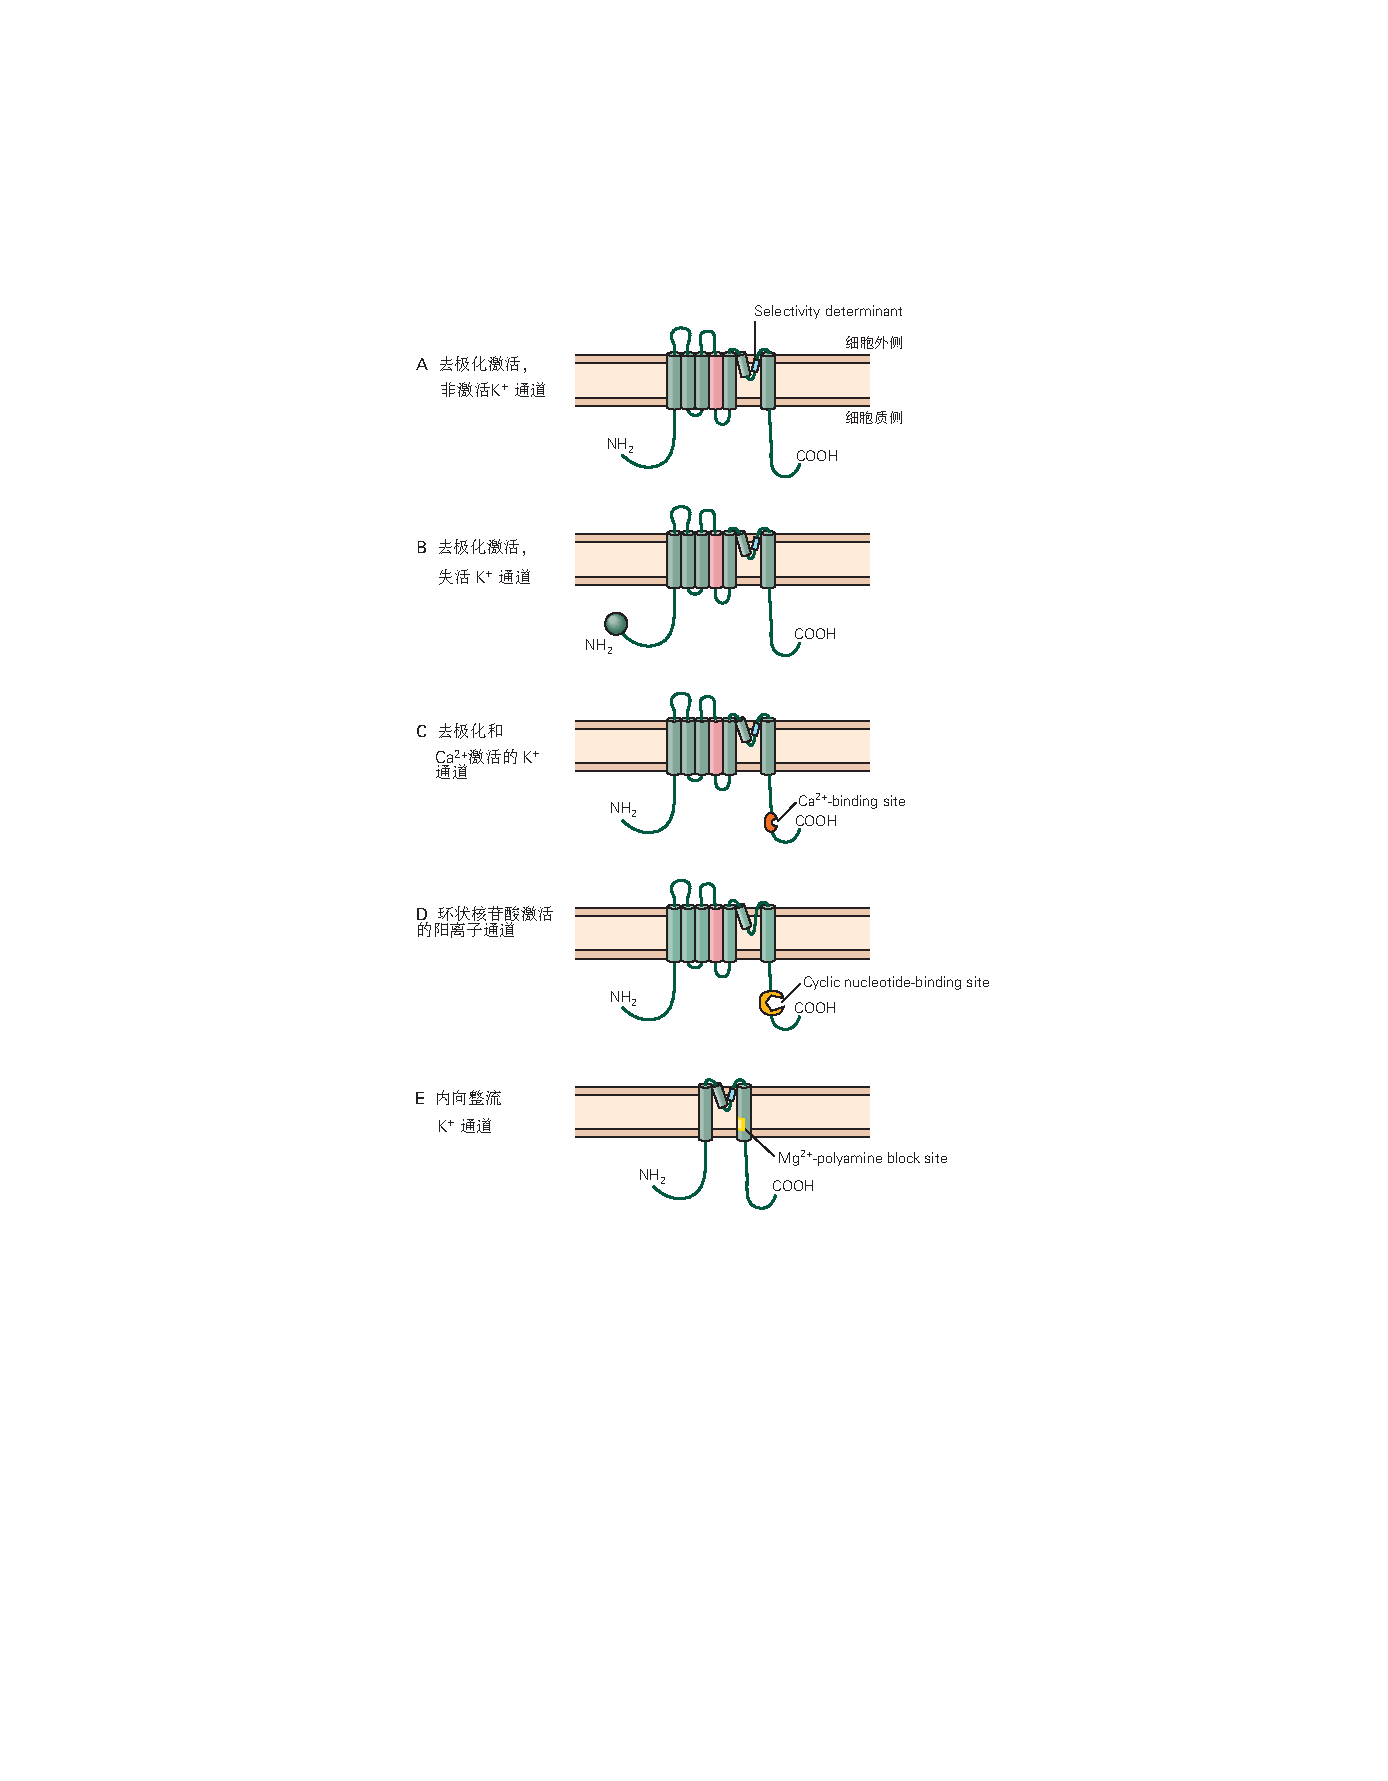
\includegraphics[width=0.6\linewidth]{chap10/fig_10_12}
	\caption{电压门控通道的扩展基因家族产生了常见分子设计的变体。 A. 电压门控 K+ 通道的 α 亚基的基本跨膜拓扑结构。 S4 跨膜 α-螺旋标记为红色。 B. 许多首先被激活然后因长时间去极化而失活的 K+ 通道在其 N 末端有一个球链片段,通过堵塞通道的内口使通道失活。 C. 一些需要去极化和细胞内 Ca2+ 增加才能激活的 K+ 通道具有连接到通道 C 末端的 Ca2+ 结合序列。 D. 由环核苷酸门控的阳离子通道具有连接到 C 末端的环核苷酸结合域。 此类通道的一个子类包括在嗅觉和视觉感觉信号的转导中很重要的电压依赖性、环核苷酸门控通道。 另一个子类包括对起搏器活动很重要的超极化激活环核苷酸门控 (HCN) 通道(参见图 \ref{fig:10_15} D)。 这些通道中的 P 环缺乏 K+ 选择性所需的关键氨基酸残基。 因此,这些通道对 Na+ 和 K+ 没有显示出高度的区分度。 E. 内向整流 K+ 通道由细胞质中可用的阻断颗粒门控,由基本构建块的截短版本形成,只有两个跨膜区域和一个 P 区域。}
	\label{fig:10_12}
\end{figure}


\begin{figure}[htbp]
	\centering
	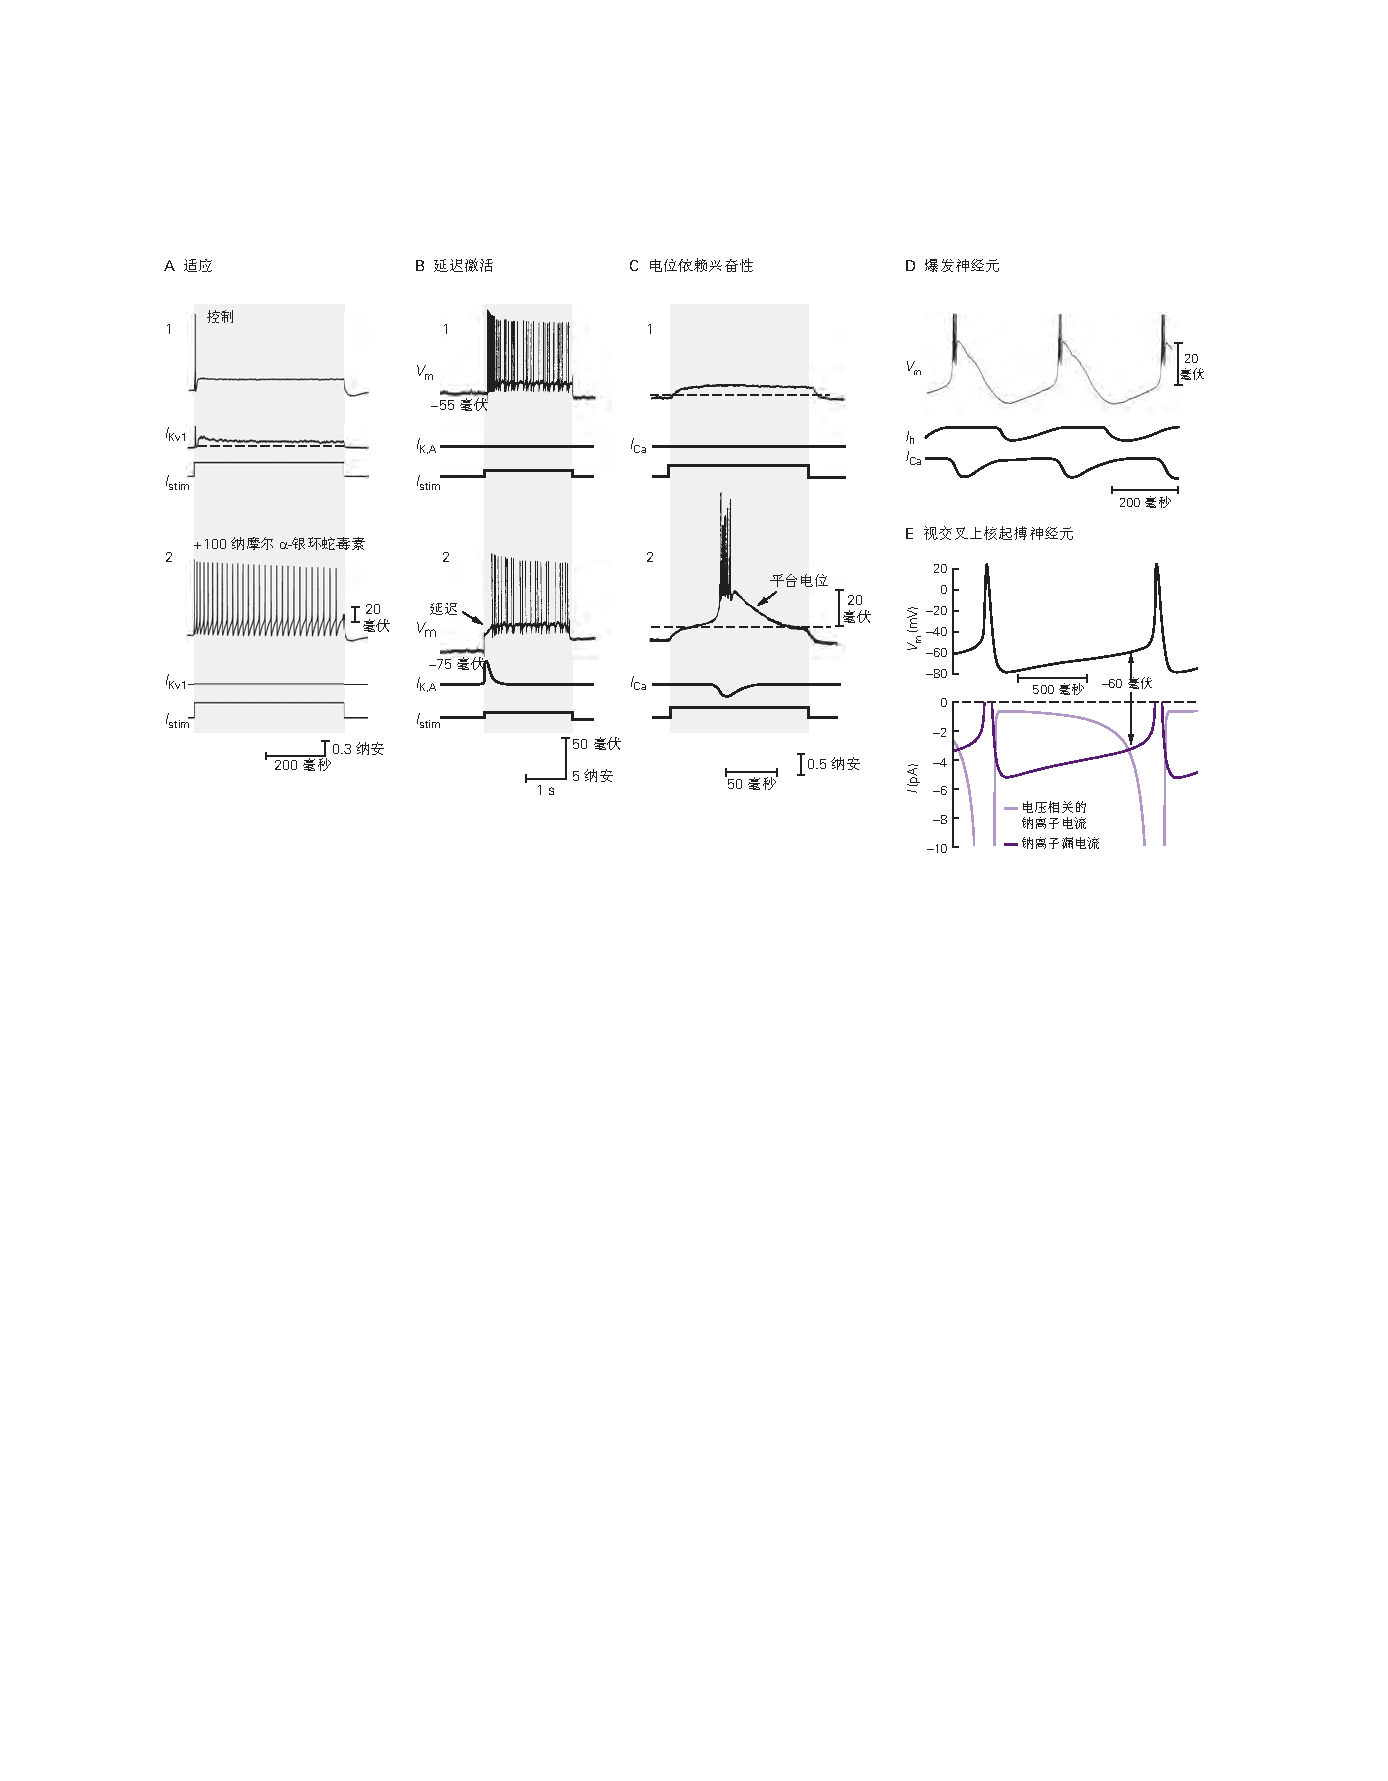
\includegraphics[width=0.85\linewidth]{chap10/fig_10_15}
	\caption{通过各种电压门控通道调节发射模式。 A. Kv1 通道的激活通常通过增加小鼠背根神经节神经元中的尖峰阈值来阻止第二动作电位的发射 (1)。 用蛇毒素 α-树毒素阻断 Kv1 通道可将激发模式从强烈适应改变为响应稳定刺激电流 (Istim) 的持续重复激发 (2)。 (来自 Pin Liu 的数据。) B. 将去极化电流脉冲 (Istim) 注入孤束核中的神经元通常会立即触发一系列动作电位 (1)。 如果细胞首先保持在超极化膜电位,则尖峰序列会延迟 (2)。 延迟是在 A 型 K+ 通道被去极化电流脉冲激活时引起的。 这些通道产生一个瞬态外向 K+ 电流 IK,A,它会短暂地减慢 Vm 接近阈值的速度。 这些通道通常在静息电位 (–55 mV) 下失活,但稳定的超极化消除了失活。 (经许可改编,摘自 Dekin 和 Getting 1987。)C. 注入静止的丘脑神经元的小去极化电流脉冲会产生亚阈值去极化 (1)。 如果膜电位保持在超极化水平,则相同的电流脉冲会触发动作电位的爆发 (2)。 电流脉冲的有效性得到增强,因为超极化导致一种电压门控 Ca2+ 通道从失活中恢复。 通过这些 Ca2+ 通道 (ICa) 去极化内向电流会产生约 20 mV 的平台电位,触发动作电位爆发。 虚线表示正常静息电位的水平。 (经 Llinás 和 Jahnsen 1982 许可改编。)B 部分和 C 部分的数据表明,稳定的超极化(例如可能由神经元的抑制性突触输入产生)可以深刻影响神经元的脉冲序列模式。 这种效应在细胞类型之间差异很大,取决于特定类型的电压门控 Ca2+ 和 K+ 通道的存在与否。 D. 在没有突触输入的情况下,丘脑皮质中继神经元可以在动作电位的短暂爆发中自发放电。 这些爆发是由电流通过两种类型的电压门控离子通道产生的。 导致爆发的逐渐去极化是由通过 HCN 通道的内向电流 (Ih) 驱动的,该通道响应超极化而打开。 突发是由通过电压门控 Cav3 通道的内向 Ca2+ 电流触发的,这些通道在相对较低的去极化水平下被激活。 这种 Ca2+ 流入产生足够的去极化以达到阈值并驱动 Na+- 依赖性动作电位的短暂爆发。 爆发期间的强烈去极化导致 HCN 通道关闭并使 Ca2+ 通道失活,从而允许超极化在发射爆发之间发展。 这种超极化然后打开 HCN 通道,启动下一个节律循环。 (经许可改编自 McCormick 和 Huguenard 1992。)E. 来自下丘脑视交叉上核的神经元产生自发的起搏器电位。 在动作电位之后,神经元自发地去极化,首先缓慢然后更快,从而产生另一个动作电位。 在尖峰间期,去极化由两个内向的 Na+ 电流驱动。 一种是“持续的 Na+ 电流”,它流经对河豚毒素阻断敏感的电压依赖性钠通道,可能与动作电位上升过程中更大的钠电流背后的通道群相同。 第二个电流流经非电压激活钠泄漏非选择性 (NALCN) 通道,该通道为 Na+ 和 K+ 离子提供稳定的电导通路。 在负电压下,Na+ 驱动力大而 K+ 驱动力小,因此漏电流主要由 Na+ 离子携带。 这种内向电流使神经元去极化,使电压依赖性持久 Na+ 电流成为主导(约 –60 mV)。 (经许可改编自 Jackson 等人,2004 年。版权所有 © 2004 神经科学协会。)}
	\label{fig:10_15}
\end{figure}


图~\ref{fig:10_12}~代表了大家族的渠道,其中有相当大的结构和功能多样性。
五种不同的机制有助于电压门控通道的多样性。


1. 多个基因编码每类通道内的相关主要亚基。
例如,在哺乳动物神经元和肌肉中,有 9 个不同的基因编码电压门控 Na+ 通道 α 亚基。


2. 形成电压门控 K+ 通道的四个 α 亚基(图 8-11)可以由不同的基因编码。
翻译后,α-亚基在某些情况下以各种组合混合和匹配,从而形成异聚通道的不同亚类。 


3. 单个基因产物可能被交替剪接,导致编码 α 亚基的信使 RNA (mRNA) 分子发生变异。


4.编码α-亚基的mRNA可以通过单个核苷酸的化学修饰进行编辑,从而改变通道亚基中单个氨基酸的组成。 


5. 所有通道类型的主要成孔 α 亚基通常与不同的辅助亚基结合,形成功能不同的通道类型。


这些辅助亚基(通常称为 β-、γ- 或 δ-亚基)可以是细胞质的或跨膜的,并且可以对通道功能产生广泛的影响。
例如,一些 β 亚基提高了通道蛋白从粗面内质网转运到细胞膜的效率,并决定了它在细胞表面的最终目的地。
其他亚基可以调节通道门控的电压灵敏度或动力学。
与 α 亚基相比,电压门控通道三个主要亚家族的 β 亚基、γ 亚基和 δ 亚基之间没有已知的同源性。


这些通道多样性的不同来源在神经系统的不同区域之间、不同类型的神经元之间以及给定神经元的不同亚细胞区室中也有很大差异。
这种区域分化的必然结果是,改变电压门控通道功能的突变或表观遗传机制可以对神经元或肌肉功能产生非常有选择性的影响。
其结果是出现了大量称为离子通道病的神经系统疾病(第 ~\ref{chap:chap57}~和~\ref{chap:chap58}~章)。



\subsection{电压门控钠通道}

哺乳动物电压依赖性 Na+ 通道的 α 亚基由九个基因编码。 由这些基因编码的三个 α 亚基(Nav1.1、Nav1.2 和 Nav1.6)在成熟哺乳动物大脑的神经元中广泛表达,而其他四个在神经元中的表达更为有限。 Nav1.3 在发育早期强烈表达,在成熟大脑中表达很少,但可以在受损组织中重新表达,例如在脊髓损伤后。 Nav1.7 通道仅限于周围神经系统中的自主神经元和感觉神经元。
Nav1.8 和 Nav1.9 通道主要局限于外围感觉神经元的一个子集,在痛觉初级感觉神经元(伤害感受器)中表现尤为突出。
与 Nav1.8 和 Nav1.9 通道相比,Nav1.1、Nav1.2、Nav1.3、Nav1.6 和 Nav1.7 通道通常具有相似的电压依赖性和相对较快的激活和失活动力学。 
骨骼肌纤维中的 Nav1.4 通道和心肌中的 Nav1.5 通道传导电压门控 Na+ 电流,从而在这些组织中产生动作电位。


Nav1.1、Nav1.2、Nav1.6虽然在哺乳动物中枢神经元中均有广泛表达,但在不同类型的神经元中表达比例不同。
Nav1.1 通道在一些抑制性 GABAergic 中间神经元中表达特别强烈,并且 Nav1.1 通道中的一些功能丧失突变可导致癫痫,如 Dravet 综合征,这可能反映了抑制性神经元相对于兴奋性神经元的兴奋性丧失更大。



\subsection{电压门控钙通道}

几乎所有神经元都包含电压门控 Ca2+ 通道,这些通道会响应膜去极化而打开。
强大的电化学梯度驱动 Ca2+ 进入细胞,因此这些通道产生内向电流,有助于使细胞去极化。


单个神经元通常表达至少四种或五种不同类型的电压门控 Ca2+ 通道,它们具有不同的电压依赖性、动力学特性和亚细胞定位。
在中枢和周围神经元中广泛表达的钙离子通道包括 Cav1.2 和 Cav1.3 通道(统称为 L 型通道)、Cav2.1(P/Q 型通道)、Cav2.2(N 型通道) ), 和 Cav2.3 (R 型通道)。
各种 Cav1 和 Cav2 家族通道统称为高阈值或高压激活 (HVA) Ca2+ 通道,因为激活通常需要相对较大的去极化。


Cav3 家族的成员,统称为 T 型或低压激活 (LVA) 通道,在某些神经元中更有选择性地表达。
它们通过小的去极化(低至 −65 mV)打开,并在数十毫秒内失活。
在正常静息电位下,Cav3 通道通常是失活的。
膜电压的超极化(如通过抑制性突触输入)消除静息失活,这使得 LVA 通道在超极化后随着膜电压移回其静息水平而瞬时激活。 
这种激活可以产生再生去极化,触发 Na+ 动作电位的爆发,当 Cav3 通道失活时终止。 
这种抑制后突发放电在丘脑的某些区域很常见,可以帮助驱动神经回路中的同步突发放电(见图 44-2)。 
在慢速起搏器电位的超极化阶段后,Cav3 通道的类似反弹激活有助于一些丘脑皮质神经元的自发节律性爆发(见图~\ref{fig:10_15})。



\subsection{电压门控钾通道}

电压依赖性 K+ 通道包含一组特别不同的通道,它们在激活动力学、电压激活范围和对各种配体的敏感性方面各不相同。
哺乳动物神经元通常表达至少五个电压依赖性 K+ 通道家族的成员:Kv1、Kv2、Kv3、Kv4 和 Kv7(图 ~\ref{fig:10_13})。
每个家族由多个基因产物组成,每个通道由四个 α 亚基组成。
例如,有八个密切相关的基因编码 Kv1 基因家族 (Kv1.1–Kv1.8) 的成员。


\begin{figure}[htbp]
	\centering
	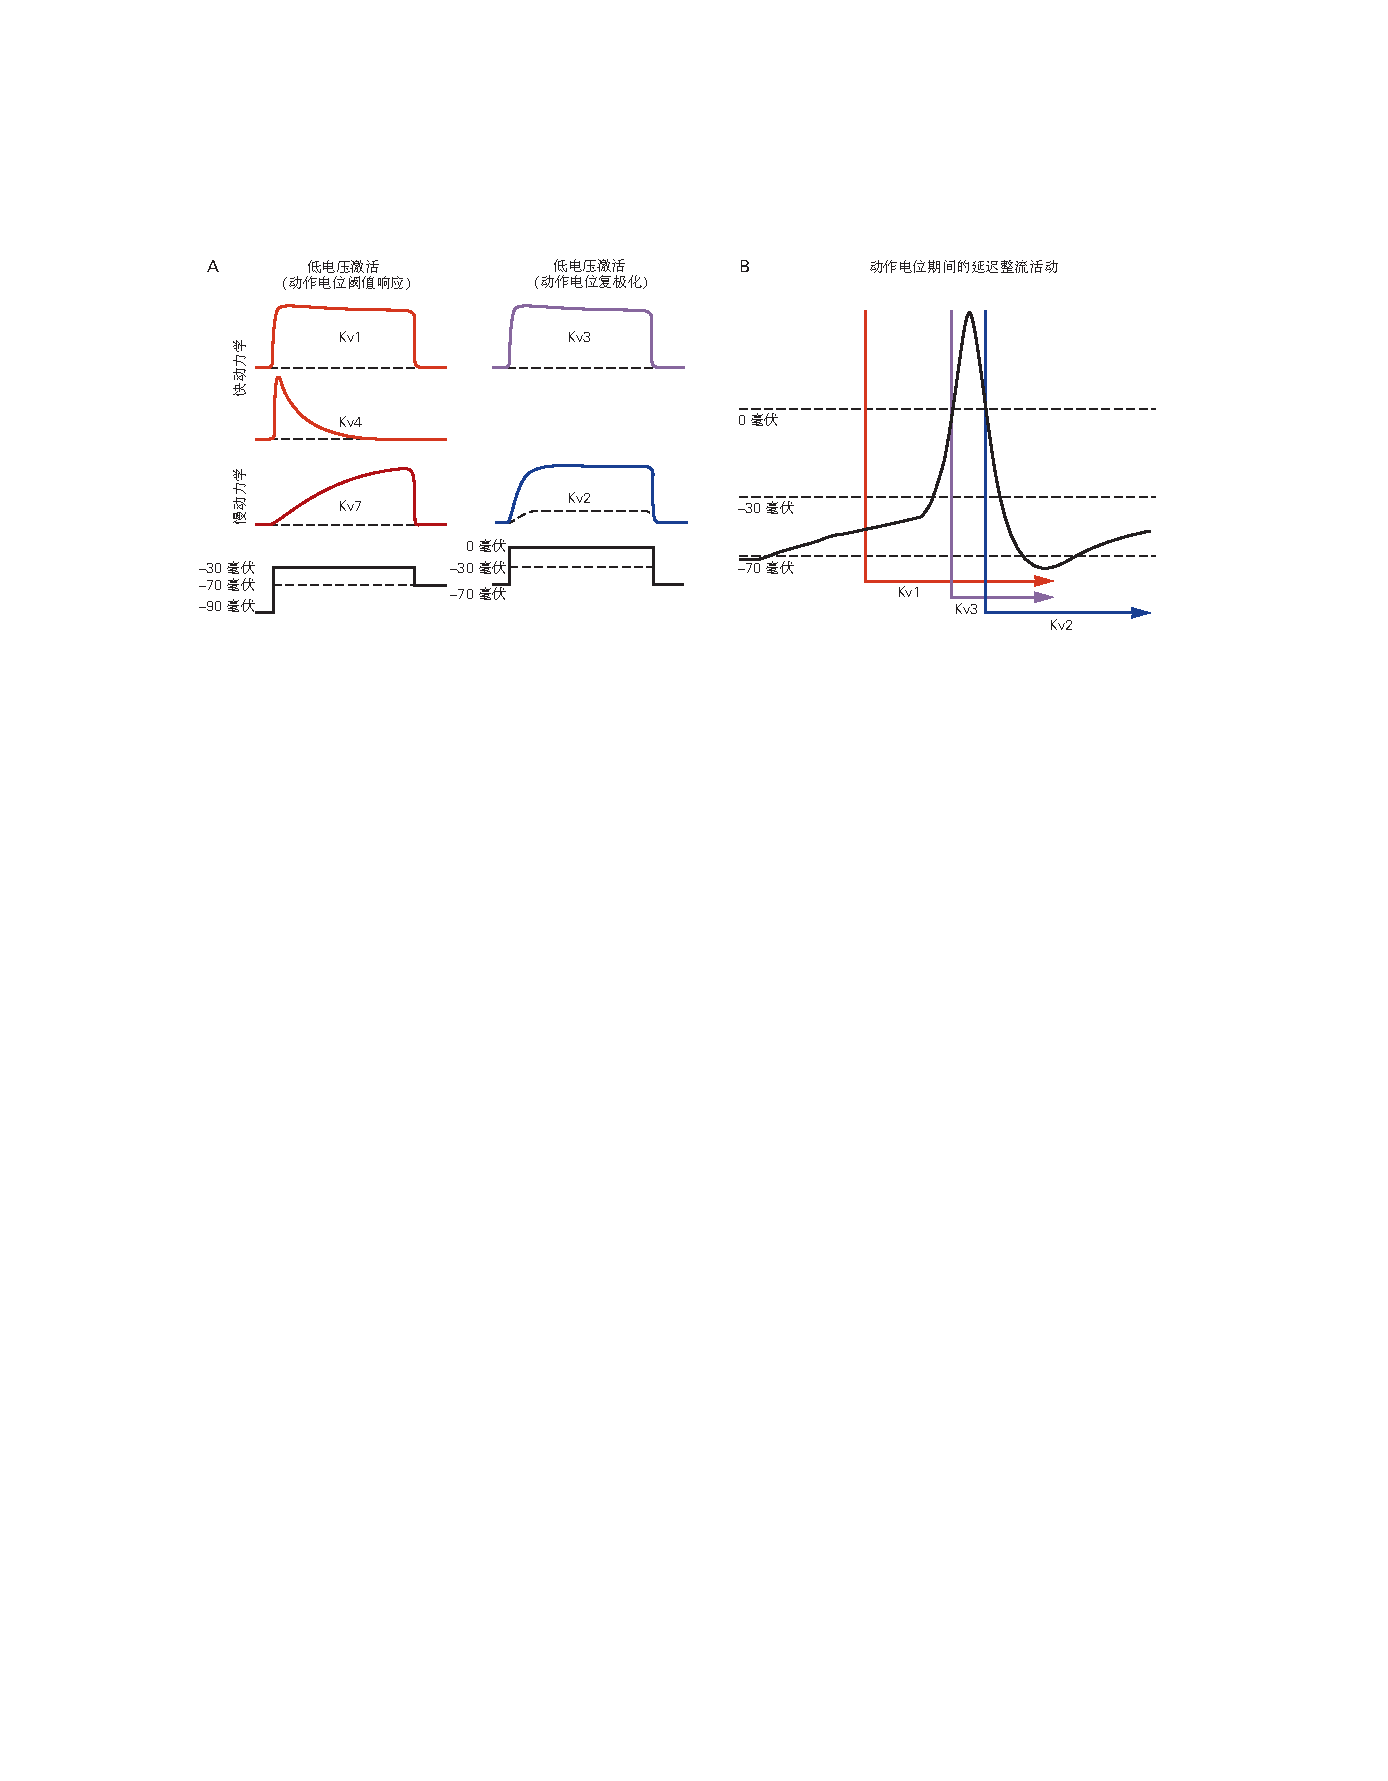
\includegraphics[width=0.8\linewidth]{chap10/fig_10_13}
	\caption{哺乳动物电压激活钾通道主要类别的不同电压依赖性和动力学。 A. 主要电压门控 K+ 家族的电压依赖性和动力学的简化概括。 由于 Kv1、Kv4 和 Kv7 通道可以被相对较小的去极化激活,因此它们通常有助于控制动作电位 (AP) 阈值。 Kv2 和 Kv3 通道需要更大的去极化才能被激活。 Kv1、Kv3 和 Kv4 通道的激活速度相对较快,而 Kv7 和 Kv2 通道的激活速度较慢。 B. 动作电位期间延迟整流 K+ 通道主要成分的不同激活时间的简化概括。 Kv1 通道需要小的去极化并且被迅速激活,有时甚至比动作电位显着提前。 Kv3 通道需要大的去极化,并且在动作电位的上升阶段后期被激活,此后非常迅速地停用。 Kv2 通道在动作电位下降阶段相对缓慢地被激活,并在后超极化期间保持开放。 (经许可改编自 Johnston 等人,2010 年。)}
	\label{fig:10_13}
\end{figure}


亚基可以是相同类型(同源通道)或来自同一 Kv 家族(异源通道)的不同基因产物。
例如,Kv1 通道可以由至少五种在中枢神经元中广泛表达的不同基因产物的异聚组合形成,每种组合具有不同的动力学和电压依赖性。
异聚通道中 α 亚基的不同组合提供的可能功能变化是巨大的,尽管并非所有可能的组合都实际发生。


区分神经元中电压依赖性 K+ 电流的不同成分的一种方法是通过是否存在失活。
非失活 K+ 电流,如 Hodgkin 和 Huxley 在鱿鱼轴突中所描述的那样,称为延迟整流 K+ 电流。
在鱿鱼轴突中,延迟整流电流流过单个 Kv1 家族通道类型。
在大多数哺乳动物神经元中,延迟整流电流包括来自 Kv1、Kv2 和 Kv3 家族通道的多个分量,每个分量具有不同的动力学和电压依赖性。
Kv3 通道在需要大量去极化才能被激活以及具有非常快速的激活动力学方面是不寻常的。
因此,Kv3 通道在动作电位接近峰值之前不会被激活,但它们的激活速度足以帮助终止动作电位。


除了延迟整流电流外,许多神经元还具有失活 K+ 电流的成分,称为 A 型电流。
在细胞体和树突中,A 型电流主要由 Kv4 家族 α-亚基形成,它们形成的通道在几毫秒到几十毫秒的时间范围内失活。
包含 Kv1.4 亚基或辅助亚基 Kvβ1 的 Kv1 通道也调节电流的失活成分,该成分在一些神经末梢和一些细胞体中高度表达。


与 Na+ 通道和 Cav3 家族通道的情况一样,A 型 K+ 电流不仅在大去极化过程中失活,而且还受到来自静止的小去极化的稳态失活,提供了一种可以通过小电压变化调制其幅度的机制 围绕静息电位(参见图~\ref{fig:10_15}B)。

Kv7 亚基形成非失活通道,只需要从静息状态进行小的去极化即可激活,甚至可以在静息电位下显着激活。
在一些神经元中,Kv7 通道被通过毒蕈碱 G 蛋白偶联受体起作用的递质乙酰胆碱下调(因此另一个名称“M-current”的起源)。
Kv7 通道通常激活相对缓慢,超过数十毫秒,并且在单个动作电位期间提供很少的电流,但倾向于抑制后续动作电位的激发(第~\ref{chap:chap14}~章)。


KCNH 基因家族由三个电压门控 K+ 通道亚家族(Kv10、Kv11 和 Kv12)组成,它们也在大脑中表达。
它们影响静息电位、动作电位阈值以及放电频率和模式。



\subsection{电压门控超极化激活循环核苷酸门控通道}

许多神经元都具有被超极化缓慢激活的阳离子通道。
当细胞内环核苷酸与通道结合时,这种对超极化的敏感性会增强。
由于这些超极化激活的环核苷酸门控 (HCN) 通道在 K+ 通道的选择性过滤器中发现的四个负结合位点中只有两个,因此它们对 K+ 和 Na+ 都具有渗透性,并且具有大约 -40 到 -30 的逆转电位 毫伏。
因此,在强烈的突触抑制期间或在动作电位之后,来自静息的超极化会打开通道以产生称为 Ih 的内向去极化电流(参见图~\ref{fig:10_15}D)。



\section{细胞质钙可控制离子通道的门控}

在典型的神经元中,某些离子通道的打开和关闭可以通过各种细胞质因子进行调节,从而为神经元的兴奋性特性提供更大的灵活性。
这些细胞质因子水平的变化可能是由神经元本身的活动或其他神经元的影响引起的(第~\ref{chap:chap14}~章和第~\ref{chap:chap15}~章)。


细胞内Ca2+浓度是调节离子通道活性的重要因素之一。
虽然在动作电位期间通过膜通道的离子电流通常不会导致大多数离子种类的细胞内浓度发生明显变化,但钙是该规则的一个明显例外。
静息细胞细胞质中游离 Ca2+ 的浓度极低,约为 10-7 M,比外部 Ca2+ 浓度(大约 2 mM)低几个数量级。 
因此,由于电压门控 Ca2+ 流入,细胞内 Ca2+ 浓度可能比其静息值增加许多倍。


细胞内 Ca2+ 浓度控制许多通道的门控。
细胞内 Ca2+ 的增加激活了几种通道。
例如,在神经元中广泛表达的 Ca2+ 激活的 BK 通道(以其大的单通道电导命名)是电压依赖性 K+ 通道,在没有 Ca2+ 的情况下需要非常大的非生理去极化才能打开。
Ca2+ 与通道细胞质表面某个位点的结合会改变其电压门控,从而允许通道在更多的负电位下打开。
随着 Ca2+ 在动作电位期间的流入,BK 通道可以打开并帮助使动作电位复极化。
另一个钙激活 K+ 通道家族,SK 通道(以其小的单通道电导命名)不依赖于电压,但仅在响应细胞内 Ca2+ 增加时才打开。
SK 通道可以响应细胞内 Ca2+ 相对较小的变化而打开,但门控缓慢,因此随着更多的 Ca2+ 在重复动作电位激发过程中进入细胞,它们的激活逐渐增强。
一些 Ca2+ 通道本身对细胞内 Ca2+ 水平敏感,当细胞内 Ca2+ 由于通过通道本身进入而增加时变得失活。


如后面章节所述,细胞内 Ca2+ 浓度的变化也会影响多种细胞代谢过程,以及神经递质释放和基因表达。



\section{兴奋性特性因神经元类型而异}

通过表达不同的离子通道补充,不同神经元类型的电特性已经进化以匹配信息处理的动态需求。
因此,神经元的功能不仅由其突触输入和输出定义,而且由其内在的兴奋性特性定义。


哺乳动物神经系统中不同类型的神经元产生不同形状的动作电位,并以不同的特征模式放电,反映了电压门控通道的不同表达。
例如,小脑浦肯野神经元和 GABAergic 皮质中间神经元与 Kv3 通道的高水平表达有关。
这些通道的快速激活会产生狭窄的动作电位。
在多巴胺能神经元和其他单胺能神经元中,在动作电位下降阶段打开的电压激活 Ca2+ 通道有高水平的表达。
来自这些通道的内向 Ca2+ 电流减慢复极化,导致更宽的动作电位。


在乌贼轴突中,动作电位之后是后超极化(见图~\ref{fig:10_7})。 
在一些哺乳动物神经元中,后超极化具有持续数十甚至数百毫秒的缓慢成分,由钙激活的 K+ 通道或具有缓慢失活动力学的电压激活的 K+ 通道产生。
SK 通道介导的缓慢后超极化可以通过重复动作电位增强,反映细胞内 Ca2+ 浓度的积累。


在皮层和海马体的许多锥体神经元中,动作电位之后是后去极化,这是一种短暂的去极化,有时会在较早的后超极化之后发生。
如果后去极化足够大,它可以触发第二个动作电位,导致全或无爆发性放电。
后去极化可由多种离子电流引起,包括来自许多电压依赖性通道的 Na+ 和 Ca2+ 电流。


神经元中动作电位的形状并不总是不变的。
在某些情况下,它可以在内部(例如,通过重复放电)或外部(例如,通过突触调制)进行动态调节(第~\ref{chap:chap15}~章)。


去极化诱发的动作电位放电模式在神经元之间差异很大。 神经元的输入输出功能可以通过响应一系列不同幅度的电流注入而激发的动作电位的频率和模式来表征。
在哺乳动物的大脑皮层中,谷氨酸能锥体神经元通常在电流脉冲开始时快速放电,随后放电逐渐减慢,这种模式称为适应(图~\ref{fig:10_14}A)。
相比之下,许多 GABAergic 中间神经元的发射频率变化很小(图~\ref{fig:10_14}B)。
其他神经元具有更复杂的放电模式。
大脑皮层中的一些锥体神经元往往会随着动作电位的初始爆发而放电(图~\ref{fig:10_14}C); “喋喋不休”的细胞以反复短暂的高频发射响应(图~\ref{fig:10_14}D)。


\begin{figure}[htbp]
	\centering
	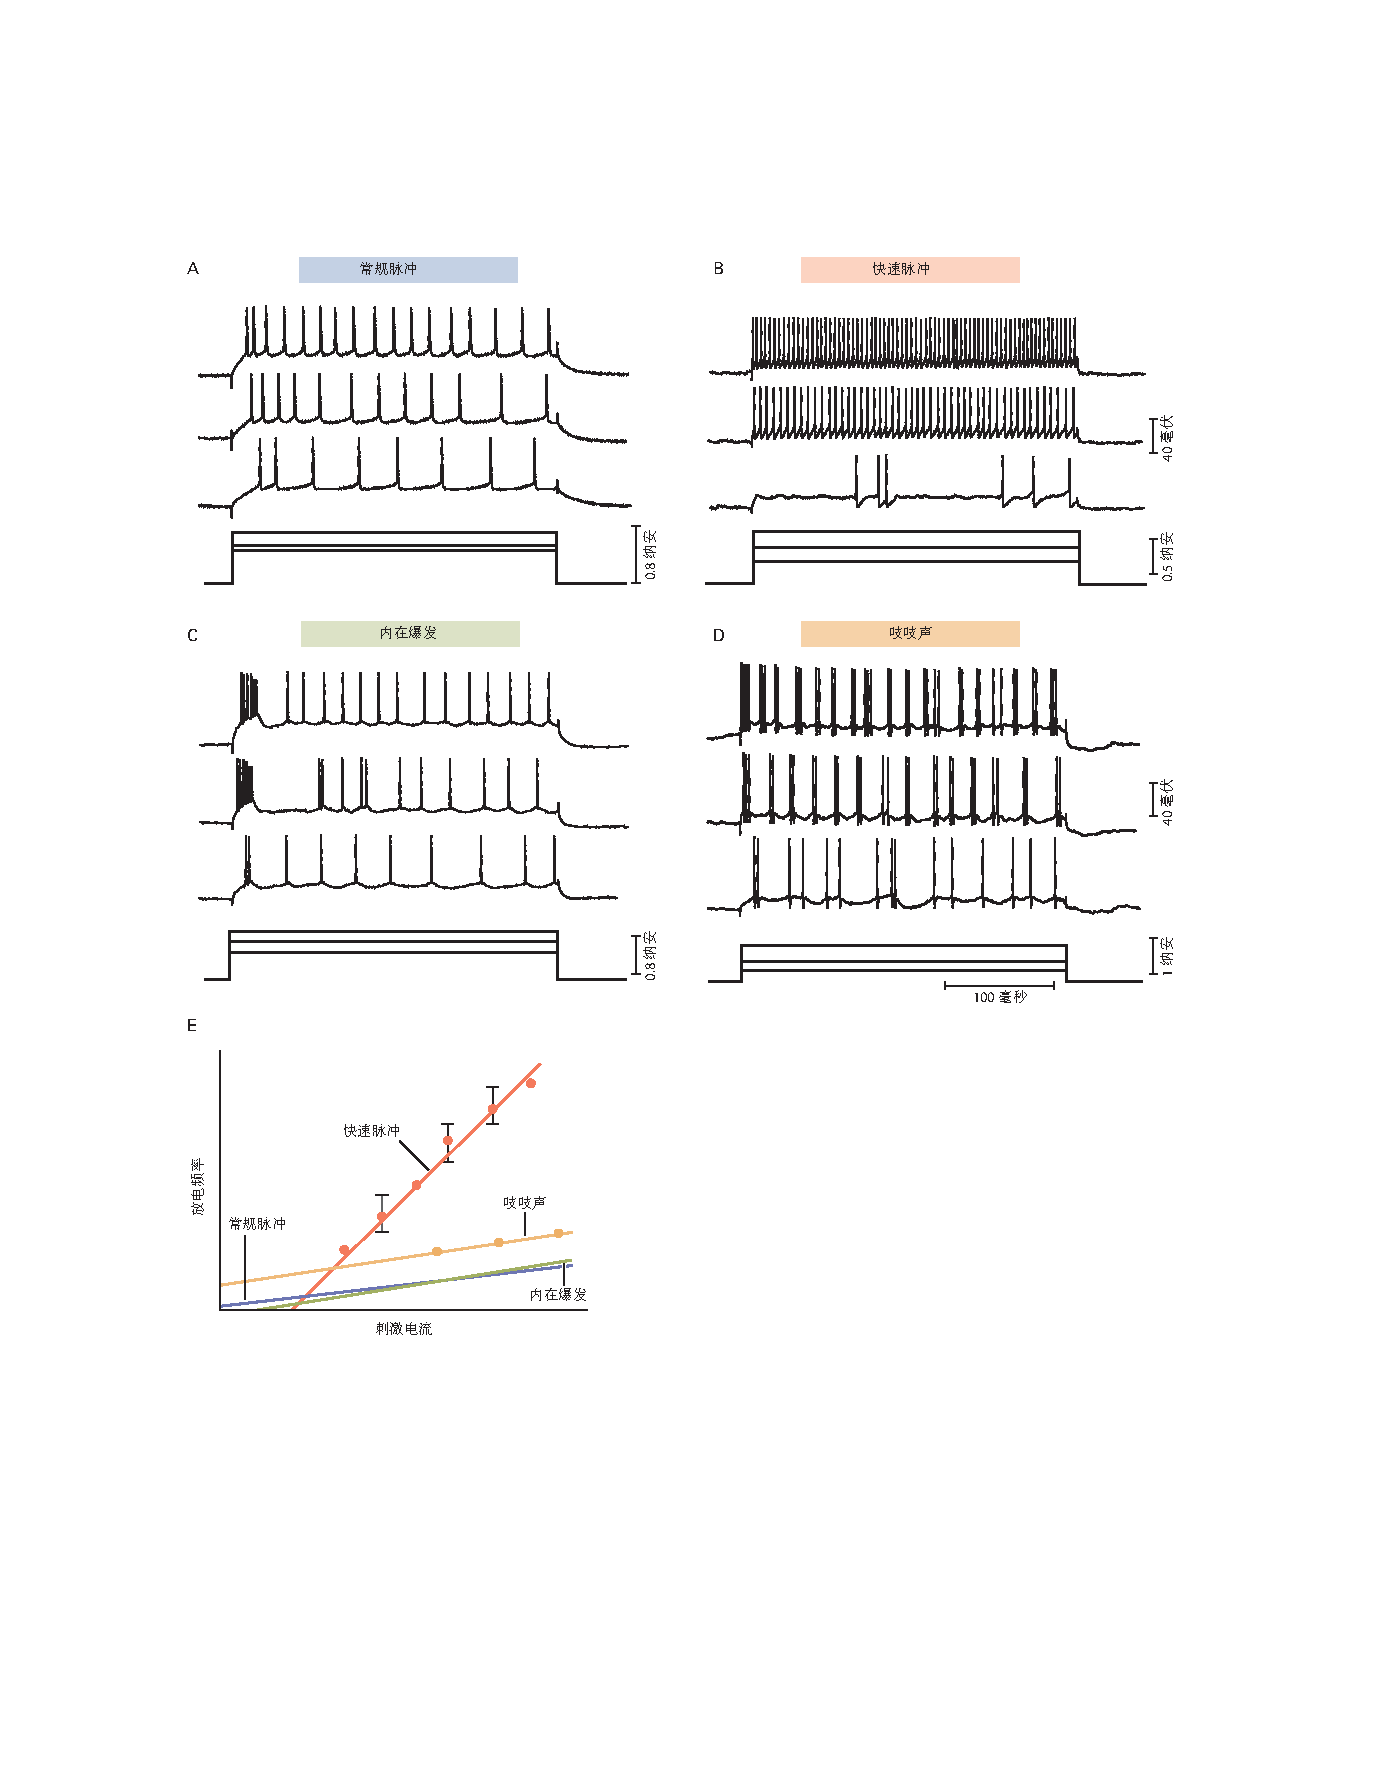
\includegraphics[width=0.75\linewidth]{chap10/fig_10_14}
	\caption{四种皮层神经元的不同放电模式。 三个步骤的去极化电流,每个具有不同的振幅,被注入每个细胞以引起放电。 (经许可改编自 Nowak 等人,2003 年。)A. 具有许多谷氨酸能皮质锥体神经元典型放电模式的皮质神经元,说明了适应性特征。 B. 许多 GABAergic 中间神经元的典型放电模式,说明维持高频重复放电。 C. 在本质上爆发的神经元中放电,这是皮质层 II/III 中锥体神经元的一种亚型。 D. 在颤振细胞中激发,皮质层中锥体神经元的一种亚型 V. E. 这四种细胞类型的激发频率与刺激电流的关系,显示出它们对增加刺激强度的不同敏感性。}
	\label{fig:10_14}
\end{figure}


这四类神经元对兴奋性输入的敏感性也可以通过它们的频率-电流关系来表征。
快速尖峰神经元对去极化兴奋电流的增加最敏感。


一些神经元可以维持高达 500 Hz 的高频重复放电。
这种快速刺激的神经元出现在整个哺乳动物的中枢神经系统中,包括听觉系统中的许多主要神经元,其中神经元必须对非常高频的声波做出反应。
以高频重复发射的能力与 Kv3 家族通道的高表达水平相关,这些通道会产生快速复极化并在复极化后极快地关闭,从而导致极小的后超极化和短暂的不应期。


神经元的不同放电模式可以根据特定通道的表达和门控特性来理解。
例如,通过激活特定的 Kv1 家族通道,可以在维持电流脉冲期间调整发射频率,这些通道在动作电位后被强烈激活,从而阻碍后续尖峰的发射(图~\ref{fig:10_15} A)。
由于许多通道都受到调节其激活可用性的失活过程的控制,因此在静息电位周围产生微小电压变化的突触输入可以极大地改变细胞的兴奋性。
例如,在某些神经元中,稳定的超极化突触输入通过降低细胞正常静息电位下 A 型 K+ 通道的失活程度,使细胞的兴奋性降低(图~\ref{fig:10_15}B)。 
在其他神经元中,这种稳定的超极化使细胞更容易兴奋,因为它减少了 Cav3 电压门控 Ca2+ 通道的失活(图 ~\ref{fig:10_15} C)。


在没有任何突触输入的情况下,哺乳动物大脑中数量惊人的神经元会自发放电。
当此类活动有规律且有节奏时,通常被称为“起搏”,类似于心脏起搏器在心脏窦房结中有节奏地自发放电。
许多释放调节性神经递质(如多巴胺、5-羟色胺、去甲肾上腺素和乙酰胆碱)的神经元会自发放电,频率通常为 0.5 至 5 Hz,导致神经元目标区域持续强直释放递质。


导致自发放电的一种机制以下丘脑视交叉上核中的神经元为例,它有助于控制整体新陈代谢和睡眠-觉醒周期的昼夜节律。
这些神经元自发地放电,白天比夜间放电更快(第 ~\ref{chap:chap44}~章)。 
这些细胞中的起搏部分由亚阈值持续 Na+ 电流驱动,这是一种小的电压依赖性电流,在负电压为 -70 mV 时流过 Na+ 通道。
该电流可以缓慢地将神经元去极化到快速动作电位激发的程度(图~\ref{fig:10_15}E)。
在相同的神经元中,存在传导 Na+“泄漏”电流的非电压依赖性通道,这会将细胞去极化到激活电压依赖性持久性 Na+ 电流的电压范围内。
这种 Na+ 泄漏通道在白天在细胞膜中的表达水平较高,导致放电率存在昼夜差异。


在黑质的多巴胺能神经元中,起搏在部分由电压依赖性 Ca2+ 电流驱动方面是不寻常的。
在神经元的生命周期中,Ca2+ 的持续进入可能导致与帕金森病中这些神经元死亡相关的代谢应激(第 ~\ref{chap:chap63}~章)。



\section{神经元区域之间的兴奋性特性不同}

神经元的不同区域具有不同类型的离子通道,支持每个区域的特殊功能。
例如,轴突起着相对简单的中继线的作用。
相比之下,神经元的输入、整合和输出区域通常在传递信息之前对它们接收到的信息执行更复杂的处理(第 ~\ref{chap:chap3}~章)。


轴突起始段的触发区具有最低的动作电位生成阈值,部分原因是它具有异常高密度的电压门控 Na+ 通道。
此外,它通常具有电压门控离子通道,对相对较小的静息电位偏差敏感。
因此,这些通道在将分级突触或受体电位转化为一系列全有或全无动作电位方面发挥着关键作用。
在许多神经元的轴突起始段高度表达的通道包括 Nav1.6、Kv1、Kv7 和低电压激活的 T 型 Ca2+ 通道。


许多类型的神经元中的树突都具有电压门控离子通道,包括 Ca2+、K+、HCN 和 Na+ 通道(第 ~\ref{chap:chap13}~章)。
当被激活时,这些通道有助于塑造突触电位到细胞体的振幅、时间过程和传播。
在一些神经元中,树突中电压门控通道的密度足以支持局部动作电位,通常具有相对较高的阈值电压。
在适度的突触刺激下,首先在轴突初始段的触发区产生完全成熟的动作电位,然后传播回树突,作为细胞已激发的突触区域的信号。


轴突下动作电位的传导主要由电压门控 Na+ 和 K+ 通道介导,其功能与鱿鱼轴突中的通道非常相似。
在有髓轴突中,Ranvier 节点具有高密度的 Na+ 通道,但具有低密度的电压激活 K+ 通道。
每个节间节段两端附近的髓鞘下有较高密度的电压激活K+通道。
这些 K+ 通道的正常功能是抑制髓鞘下轴突膜部分动作电位的产生。 
在脱髓鞘疾病中,这些通道变得暴露,因此可能会抑制裸轴突传导动作电位的能力(第~\ref{chap:chap9}~章和第~\ref{chap:chap57}~章)。


化学突触处的突触前神经末梢具有高密度的电压门控 Ca2+ 通道,最常见的是 Cav2.1(P/Q 型)通道、Cav2.2(N 型)通道或两者的混合。
到达终端的动作电位会打开这些通道,导致 Ca2+ 流入,从而触发递质释放(第~\ref{chap:chap15} ~章)。



\section{神经元兴奋性是可塑的}

电压门控离子通道的表达、定位和功能状态在特定神经元中控制动作电位放电的速率和模式并不总是固定的,但会随着神经元突触输入、其活动或其活动的变化而变化 环境,以及对伤害或疾病的反应。
例如,通过第二信使通路引起通道磷酸化的突触输入可导致通道功能特性的瞬时变化,进而调节细胞兴奋性(第 ~\ref{chap:chap14}~章)。 
可塑性也可以在更长的时间尺度上发生,例如当神经元网络作为一个整体的活动增加导致单个神经元的兴奋性降低时——一种稳态反馈系统。
在某些情况下,活动引起的结构变化,例如轴突起始段长度的变化或其相对于体细胞的迁移,也会影响兴奋性。
神经元兴奋性稳态变化的分子机制尚不清楚,但可能涉及控制特定离子通道转录或细胞运输的细胞内钙信号通路。 
这种调节通路的功能障碍可能是某些类型的癫痫和与神经性疼痛等病症相关的过度兴奋的基础。




\section{亮点}

1. 动作电位是离子通过电压门控通道穿过细胞膜并因此改变跨膜电荷分离时产生的持续约 1 毫秒的膜电压瞬时去极化。 


2. 动作电位的去极化阶段是由电压激活的 Na+ 通道快速、再生性打开引起的。
复极化是由于 Na+ 通道的失活和 K+ 通道的激活。 


3. 动作电位产生的尖锐阈值发生在内向 Na+ 通道电流刚好超过通过泄漏通道和电压门控 K+ 通道的外向电流的电压处。


4. 不应期反映动作电位后Na+通道失活和K+通道持续激活。
不应期限制动作电位放电率。 


5. 电压依赖性激活和失活的通道蛋白构象变化尚未完全了解,但已确定参与通道门控的关键区域。


6. 电压门控钠通道根据离子的大小、电荷和水合能量选择钠。


7. 大多数神经元表达多种电压门控 Na+、Ca2+、K+、HCN 和 Cl- 通道,尤其是 K+ 通道的特性差异很大。 


8. 电压依赖性通道的多样性反映了多种基因的表达、多种基因产物异聚通道的形成、基因转录物的可变剪接、mRNA 编辑以及成孔亚基与多种辅助蛋白的结合。


9. 一些电压门控离子通道的活性可以通过细胞质 Ca2+ 进行调节。


10. 电压门控离子通道表达的多样性导致不同类型神经元和同一神经元不同区域的兴奋性特性不同。


11. 离子通道的区域表达和功能状态可以根据细胞活动、细胞环境变化或病理过程进行调节,从而导致神经元内在兴奋性的可塑性。


